\documentclass{vldb}

\usepackage{booktabs} % For formal tables
\usepackage{amsmath}
\usepackage{graphicx,xspace,verbatim,comment}
\usepackage{hyperref,array,color,balance,multirow}
\usepackage{balance,float,url,amsfonts,alltt}
\usepackage{mathtools,rotating,amsmath,amssymb}
\usepackage{color,ifpdf,fancyvrb,array}
% \usepackage{algorithm,algpseudocode}
\usepackage{etoolbox,listings,subcaption}
\usepackage{bigstrut,morefloats}
%\usepackage[linesnumbered,boxruled]{algorithm2e}
\usepackage[boxruled]{algorithm2e}
\usepackage{pbox}

\DeclarePairedDelimiter{\ceil}{\lceil}{\rceil}
\DeclarePairedDelimiter{\floor}{\lfloor}{\rfloor}

\newcommand{\eat}[1]{}
\newcommand{\red}{\textcolor{red}}

\newenvironment{packeditems}{
\begin{itemize}
  \setlength{\itemsep}{1pt}
  \setlength{\parskip}{0pt}
  \setlength{\parsep}{0pt}
}{\end{itemize}}

\newenvironment{packedenums}{
\begin{enumerate}
  \setlength{\itemsep}{1pt}
  \setlength{\parskip}{0pt}
  \setlength{\parsep}{0pt}
}{\end{enumerate}}

% \setcopyright{rightsretained}

\title{Are Joins Safe to Avoid for High-Capacity Classifiers?\\(Experiments and Analysis)}

\numberofauthors{1}
\author{
\alignauthor Vraj Shah$^1$\hspace{20mm}Arun Kumar$^1$\hspace{20mm}Xiaojin Zhu$^2$\\
\affaddr{\vspace{2mm}$^1$University of California, San Diego\hspace{20mm}$^2$University of Wisconsin-Madison}
\email{\{vps002, arunkk\}@eng.ucsd.edu, jerryzhu@cs.wisc.edu}
}

\begin{document}

\maketitle

\begin{abstract}
Machine learning (ML) over relational data is a booming area of the database industry and 
academia. While several projects aim to make ML scalable and fast, little work has 
addressed the pains of \textit{sourcing} data and features for ML tasks. 
Real-world relational databases typically have many tables (often, dozens) and data scientists 
often struggle to even obtain and join all possible tables that provide features for ML. 
In this context, Kumar et al.~showed recently that key-foreign key dependencies (KFKDs) 
between tables often lets us avoid such joins without significantly affecting prediction 
accuracy--an idea called ``avoiding joins safely." While initially controversial, that idea has since 
been used by various companies to reduce the burden of data sourcing.
But this prior work applied only to simple linear classifiers. In this work, we verify if their results 
hold true for a few popular complex classifiers: decision trees, SVMs, and ANNs. We conduct an 
extensive experimental study using both real-world datasets and simulations to analyze the 
effects of avoiding KFK joins on such models. Our results show that these high-capacity classifiers are 
surprisingly and counter-intuitively \textit{more} robust to avoiding KFK joins compared to linear 
models! We explain this behavior intuitively and identify open questions at the intersection 
of data management and ML theoretical research. All code and data used in this experimental 
study are available for download from \url{http://cseweb.ucsd.edu/~arunkk/hamlet}.
%We also identify and resolve two key 
%practical bottlenecks in using foreign keys as features for decision trees.
\end{abstract}

\section{Introduction}

However, from conversations with data 
scientists in practice, we learned that they often end up spending a bulk of their time on just
\textit{data sourcing}--obtaining and curating relevant features for their ML tasks, even 
before the training process can begin. Unfortunately, little work in our community has studied 
how to exploit the fundamental properties of relational data and the behavior of ML models in 
order to help reduce the burden of data sourcing.


Real-world relational databases typically have many tables connected by \textit{database dependencies}~\cite{cowbook}. Thus, a common pre-processing step 
performed by data scientists before building a machine learning (ML) model is to \textit{join} all tables they think might provide 
``useful'' features~\cite{crossmine,orion,rendle,hamlet,olteanuf}.
In general, a join might duplicate records in the training set and violate the ``IID'' sampling assumption~\cite{hastie}. 
In response, ``non-IID'' statistical relational learning (SRL) models have been studied extensively~\cite{srlbook}. 
However, an important class of problems have fallen through the cracks in this dichotomy: 
joins that do \textit{not} duplicate records, viz., \textit{key-foreign key} (KFK) joins, and thus, do not technically violate the IID sampling assumption.

\paragraph*{Example (based on~\cite{orion})}
Consider an insurance data scientist using ML for a common classification task: predicting \textit{customer churn}. She starts with the main table (simplified 
for exposition): \texttt{Customers} (\underline{\texttt{CustomerID}}, \texttt{Churn}, \texttt{Gender}, \texttt{Age}, \texttt{Employer}). 
\texttt{Churn} is the target, while \texttt{Gender}, \texttt{Age}, and \texttt{Employer} are features. So far, this is a standard classification task.  
But then, she notices the table \texttt{Employers} (\underline{\texttt{Employer}}, \texttt{State}, \texttt{Revenue}) in her database with extra features about 
customers' employers (e.g., Google or Microsoft). \texttt{Customers}.\texttt{Employer} is then a \textit{foreign key} that connects these two tables. 
She joins the tables to bring in the extra features because she has a hunch that customers employed by rich corporations in coastal states might be less likely 
to churn. She then tries various classifiers, e.g., logistic regression or decision trees.

The above join is a KFK join that does not duplicate records: a customer has exactly one employer (but many customers might have the same employer).
SRL is an overkill for this setting because the features brought in by a KFK join, which we call \textit{foreign features}, are just \textit{functions} of 
the foreign key feature; in database parlance, this is a \textit{functional dependency} (FD)~\cite{cowbook}.\footnote{Strictly speaking, an FD is different 
from a Key-Foreign Key Dependency (KFKD)~\cite{dbtheorybook}, but for most practical purposes in ML, KFKDs behave just like FDs~\cite{hamlet}.} 
An FD is to a categorical feature what an arithmetic function (e.g., square) is to a numeric feature. But foreign features typically provide a far more 
\textit{coarse-grained view} than the foreign key feature.
Our example is not a one-off; KFK joins are ubiquitous across domains, including insurance, retail, telecommunications, Web security, 
and e-commerce. In fact, from conversations with many data scientists in such domains, we learned that they routinely perform KFK joins before using 
regular ML classifiers (Section 3 gives more examples). To introduce some terminology, the main table (e.g., \texttt{Customers}) is often called the 
\textit{fact table}, while a table with foreign features (e.g., \texttt{Employers}) is called a \textit{dimension table}~\cite{cowbook}.
%
The coarse granularity of foreign features could indeed help \textit{interpretability}. But from a pure \textit{accuracy} (generalization) perspective, 
an interesting question to answer is: 

\begin{center}\textit{Are foreign features really ``needed'' to improve ML accuracy?}\end{center}

At first glance, this question might seem surprising and counter-intuitive. Why discard foreign features a priori? Why will foreign features 
behave any differently than other features? 

The answer to the first question is clear: avoiding extra foreign features reduces the total number of features \textit{without running any computations}, 
which reduces the runtimes of ML and feature selection methods~\cite{guyon}; moreover, join computation times are also saved. 
Furthermore, worrying about fewer tables (and features) could help data scientists' productivity. For example, our conversations revealed that often, different tables 
are ``owned'' by different teams even within the same company, which causes logistical headaches for data scientists even to procure those extra dimension tables.

The answer to the second question relies on an obvious but key fact: \textit{given the foreign key, all foreign features are fixed} (the very definition of an FD!).
Formally, foreign features are \textit{redundant}, given the foreign key. 
So, a tempting conclusion is that foreign features (and such KFK joins) are never needed for accuracy! Alas, recent work poured cold water
on this possibility: using a foreign key feature instead of foreign features often causes extra \textit{overfitting} even for simple \textit{linear} VC-dimension classifiers,
e.g., logistic regression and Naive Bayes~\cite{hamlet}. This is because foreign key features typically have much larger domains than foreign features (e.g., 
\texttt{Employer} has thousands of values but \texttt{State} has only a few dozen). 
Only when the number of training examples is far higher than the number of foreign key values ($>20$x) does the extra overfitting subside.

\textit{In this paper, we revisit the above question of whether foreign features are needed for accuracy for two popular \textit{high capacity} classifiers: 
decision tree and SVM with RBF kernel.}

The natural expectation is that these complex models, which have infinite VC dimensions, might face even higher overfitting than linear models if foreign features are 
discarded. In this paper, we show that surprisingly, their behavior is the \textit{exact opposite}! We start by presenting empirical results 
on the real datasets with KFK joins from~\cite{hamlet}. For both classifiers, it turns out that in \textit{almost all cases}, dimension tables can be safely 
discarded. In contrast, for linear classifiers, they could be discarded in only half of the cases.

To understand the above surprising behavior in depth, we conduct an extensive simulation study using a decision tree. We generate data for a two-table KFK join 
and embed various ``true'' distributions for the target. This includes a known ``worst-case'' scenario for discarding foreign features a priori when learning a linear model, 
i.e., the (holdout) test errors blow up~\cite{hamlet}. We vary different properties of the data and the true distribution: 
numbers of features in each base table, numbers of training examples, foreign key domain size, noise in the data, and foreign key skew. 
In very few of these cases does discarding foreign features cause the error to rise beyond $1\%$! Indeed, the only scenario where discarding foreign features seems to increase 
overfitting significantly is when the number of training examples is less than $3$x the number of foreign key values. This scenario arose in only one of the seven real datasets.
These results are in stark constrast to the results for linear models.

Our counter-intuitive results raise open questions for ML theoretical research about why decision trees and RBF-SVMs are so much more robust to discarding foreign features
than linear models. As a step in this direction, we provide some intuitive explanations that shed some light into their behavior. 
Essentially, we explain why RBF-SVMs with foreign key features behave somewhat like a 1-nearest neighbor classifier due to the high dimensionality of foreign key features with 
one-hot encoding. While this leads to a form of \textit{memorization} of the foreign key's domain, this seems to have little effect on the model's generalization or test errors.
This is similar to how memorization seems to occur in deep neural networks~\cite{rechtdnn}, but a key difference in our setting is that such memorization does not apply to
\textit{all} features. We also discuss why decision trees are robust to operating with foreign key features. 
Still, many open questions remain and we hope our results contribute to more discussions and research on this topic.

\eat{
We extend the worst-case simulation scenario for linear models by replicating the foreign feature that determines the target multiple times. The idea is to make a model that uses 
the foreign key feature alone to overfit more than one that uses the foreign features. In particular, for the RBF-SVM, this scenario demonstrates that it behaves 
more similarly to a 1-nearest neighbor classifier when using the foreign key feature but less so when the number of relevant foreign features are increased.
}

Finally, from follow-up conversations with some data scientists, we learned that while they found foreign key features to be helpful for accuracy, they faced two new practical 
bottlenecks when using them for decision trees. The first is that the sheer size of a foreign key feature's domain makes it hard to interpret and visualize the trees. 
The second is that some foreign key values may not have any training examples even if they are known to be in the domain. 
We propose simple but effective heuristics to handle these bottlenecks and make foreign key features more practical. For the first bottleneck, we propose simple lossy 
\textit{domain compression} methods that are configurable with a user-given size budget. For the second bottleneck, we propose a form of foreign key \textit{smoothing} 
that exploits foreign features as side information. We validate the accuracy of these techniques using both real and synthetic datasets.

\vspace{1mm}
\noindent Overall, the contributions of this paper are as follows:

\begin{packeditems}
\item To the best of our knowledge, this is the first paper to study the effects of discarding foreign features and KFK joins on high capacity classifiers.
We present an empirical study with several real-world datasets that shows that decision trees and RBF-SVMs are surprisingly robust to discarding foreign features a priori.

\item We conduct a comprehensive and in-depth simulation study with a decision tree to assess the effects of different data properties on how safe foreign features are to discard.

\item We take a step towards formally analyzing the behavior of decision trees and RBF-SVMs in our setting and identify some open questions for ML theoretical research.

\item We identify two practical bottlenecks with foreign key features and resolve them with simple but effective heuristics.
\end{packeditems}


\paragraph*{\textbf{Outline}} In the rest of this section, we discuss related prior work and position our work. Section 2 presents our notation, scope, and assumptions. 
Section 3 presents results on the real data. Section 4 presents our in-depth simulation study and analysis. Section 5 presents our techniques to make foreign key features
more practical. %We conclude in Section 6.

\section{Preliminaries}
% We now explain our problem setting and notation, followed by an example. We then explain our assumptions and scope.

\subsection{Notation}
The setting we focus on is the following: the dataset has a set of tables in the \textit{star schema} with KFK dependencies (KFKDs).
Star schemas are ubiquitous in many applications~\cite{cowbook}.
The fact table, which has the target variable, is denoted \textbf{S}. It has the schema $\textbf{S}(\underline{SID},Y, \textbf{X}_S, FK_1, \dots, FK_q)$.
A dimension table is denoted $\textbf{R}_i$ ($i = 1$ to $q$) and it has the schema $\textbf{R}_i(\underline{RID_i},\textbf{X}_{R_i})$.
$Y$ is the target variable (class label), $\textbf{X}_S$ and $\textbf{X}_{R_i}$ are vectors (sequences) of features, $RID_i$ is the primary key
of $\textbf{R}_i$, while $FK_i$ is a foreign key feature that refers to $\textbf{R}_i$. We call $\textbf{X}_S$ \textit{home} features and $\textbf{X}_{R_i}$ \textit{foreign} features.
For ease of exposition, we also treat \textbf{X} as a \textit{set} of features since the order among features is immaterial in our setting.
Let \textbf{T} denote the output of the projected equi-join (key-foreign key, or KFK for short) query that constructs the full training dataset by 
\textit{concatenating} the features from all base tables: $\textbf{T} \leftarrow \pi(\textbf{R} \bowtie_{RID=FK} \textbf{S})$. In general, its schema is 
$\textbf{T}(\underline{SID},Y,\textbf{X}_S,FK_1,\dots,FK_q,\textbf{X}_{R_1},\dots,\textbf{X}_{R_q})$. In contrast to our setting, traditional ML 
formulations do not distinguish between home features, foreign keys, and foreign features. The number of tuples in \textbf{S} (resp.~\textbf{R}) is 
denoted $n_S$ (resp.~$n_R$); the number of features in $\textbf{X}_S$ (resp.~$\textbf{X}_R$) is denoted $d_S$ (resp.~$d_R$). Without loss of generality, we
assume that the join is not selective, which means $n_S$ is also the number of tuples in \textbf{T}. $\mathcal{D}_{FK}$ denotes the domain of $FK$ 
and by definition, $|\mathcal{D}_{FK}| = n_R$. We call $\frac{n_S}{n_R}$ the \textit{tuple ratio}.
\eat{\footnote{Note that this setting is 
different from the statistical relational learning (SRL) setting in which the joins could violate the IID assumption because they are not KFK (labeled examples in \textbf{S}
might get duplicated. KFK joins do not cause such repetitions.}}

\eat{
\paragraph*{Example}
Consider a common classification task for which ML classifiers are used, predicting \textit{customer churn}.
The fact table is \texttt{Customers} (\underline{\texttt{CustomerID}}, \texttt{Churn}, \texttt{Gender}, \texttt{Age}, \texttt{Employer}, \texttt{ZipCode}).
\texttt{Employer} and \texttt{Zipcode} are foreign key features that refer respectively to a customer's employer (e.g., Google or Microsoft) and the area 
where a customer lives. The respective dimension tables are \texttt{Employers} (\underline{\texttt{Employer}}, \texttt{State}, \texttt{Revenue}) 
and \texttt{Areas} (\underline{ZipCode}, \texttt{CrimeRate}, \texttt{AccidentRate}).
In such scenarios, data scientists typically join all base tables to bring in the extra features from the dimension tables. In this case, they might do so 
because of a hunch that customers employed by rich corporations in coastal states and living in ``safe'' areas are unlikely to churn.
}

\subsection{Assumptions and Scope}
For the sake of tractability, in this paper, we adopt some of the same assumptions as~\cite{hamlet}. In particular, we assume the features are 
\textit{categorical} (nominal). Numeric features can be pre-discretized using standard techniques, e.g., unsupervised binning~\cite{mitchellbook}. 
Interestingly, this assumption is implicitly unavoidable for $X_R$ due to the presence of the FD $FK \rightarrow X_R$. If binning is not done for 
numeric feature in $X_R$, it ``behaves" as a categorical feature whose domain could be as large as $\mathcal{D}_{FK}$.
We also focus on binary classification but our ideas can be easily applied to 
multi-class targets as well. We assume that the foreign key features ($FK_i$) are not (primary) keys in the fact table, e.g., \texttt{Employer} does 
not uniquely identify a customer.\footnote{Primary keys in the fact table are \textit{not} generalizable features, unlike foreign keys.}
Finally, we also do not study the ``cold start'' issue because it is orthogonal to the focus of this paper~\cite{coldstart}. In other words, we assume that all features 
have known finite domains, possibly including a special ``Others'' placeholder to temporarily handle hitherto unseen values. In our example, this means that both 
\texttt{Employer} and \texttt{Gender} have known finite domains. In general, $FK_i$ can take values only from the given set of $\textbf{R}_i.RID_i$ values 
(new $FK_i$ values are mapped to ``Others''). Since ML models are rebuilt periodically in practice, new information can then be added to expand feature domains. 
We emphasize that our goal is \textit{not} to create new classification or feature selection algorithms, nor is to compare which algorithms yield lowest errors.
Our goal is to expose and analyze how KFKDs/FDs enable us to dramatically discard foreign features a priori when learning two popular high capacity 
classifiers: decision tree (CART), RBF-SVM.


\begin{table}[t]
\centering
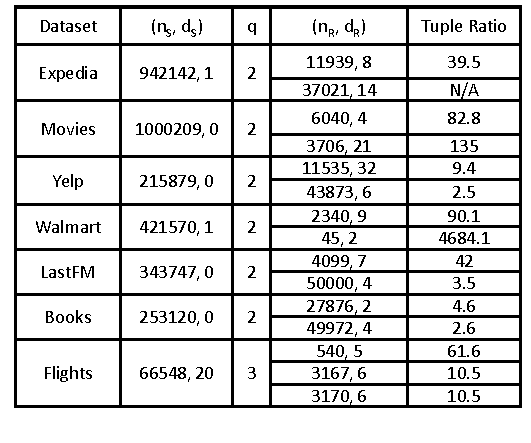
\includegraphics[width=0.99\linewidth]{table1.pdf}
\caption{Dataset statistics. $q$ is the number of dimension tables. All features are categorical. $n_S$ is the number of labeled examples, also 
overloaded to mean the number of training examples ($50\%$ as many). So, the tuple ratio here is actually $50\% \times n_S / n_R$. N/A means the 
corresponding dimension table can never be discarded because its corresponding foreign key has an ``open'' domain.
}
\label{Table:datastats}
\end{table}


\section{Empirical Study with Real Data}

\subsection{Datasets}
We take the seven real datasets from~\cite{hamlet}; these are originally from Kaggle, GroupLens, \url{openflights.org}, \url{mtg.upf.edu/node/1671}, and \url{last.fm}.
Two datasets have binary targets (Flights and Expedia); the others have multi-class ordinal targets. For the sake of simplicity, we binarize all targets 
for this paper by grouping ordinal targets into lower and upper halves (this change does not affect our overall conclusions). 
The dataset statistics are provided in Table~\ref{Table:datastats}. 
We briefly describe the task for each dataset and explain what the foreign features are. More details about their schemas, including the list 
of all features are already in the public domain (listed in~\cite{hamlet}). 
\textit{All of our datasets, scripts, and code will be made available on our project webpage\footnote{\url{http://cseweb.ucsd.edu/~arunkk/hamlet}} to make reproducibility easier.}


\begin{table*}[t]
\centering
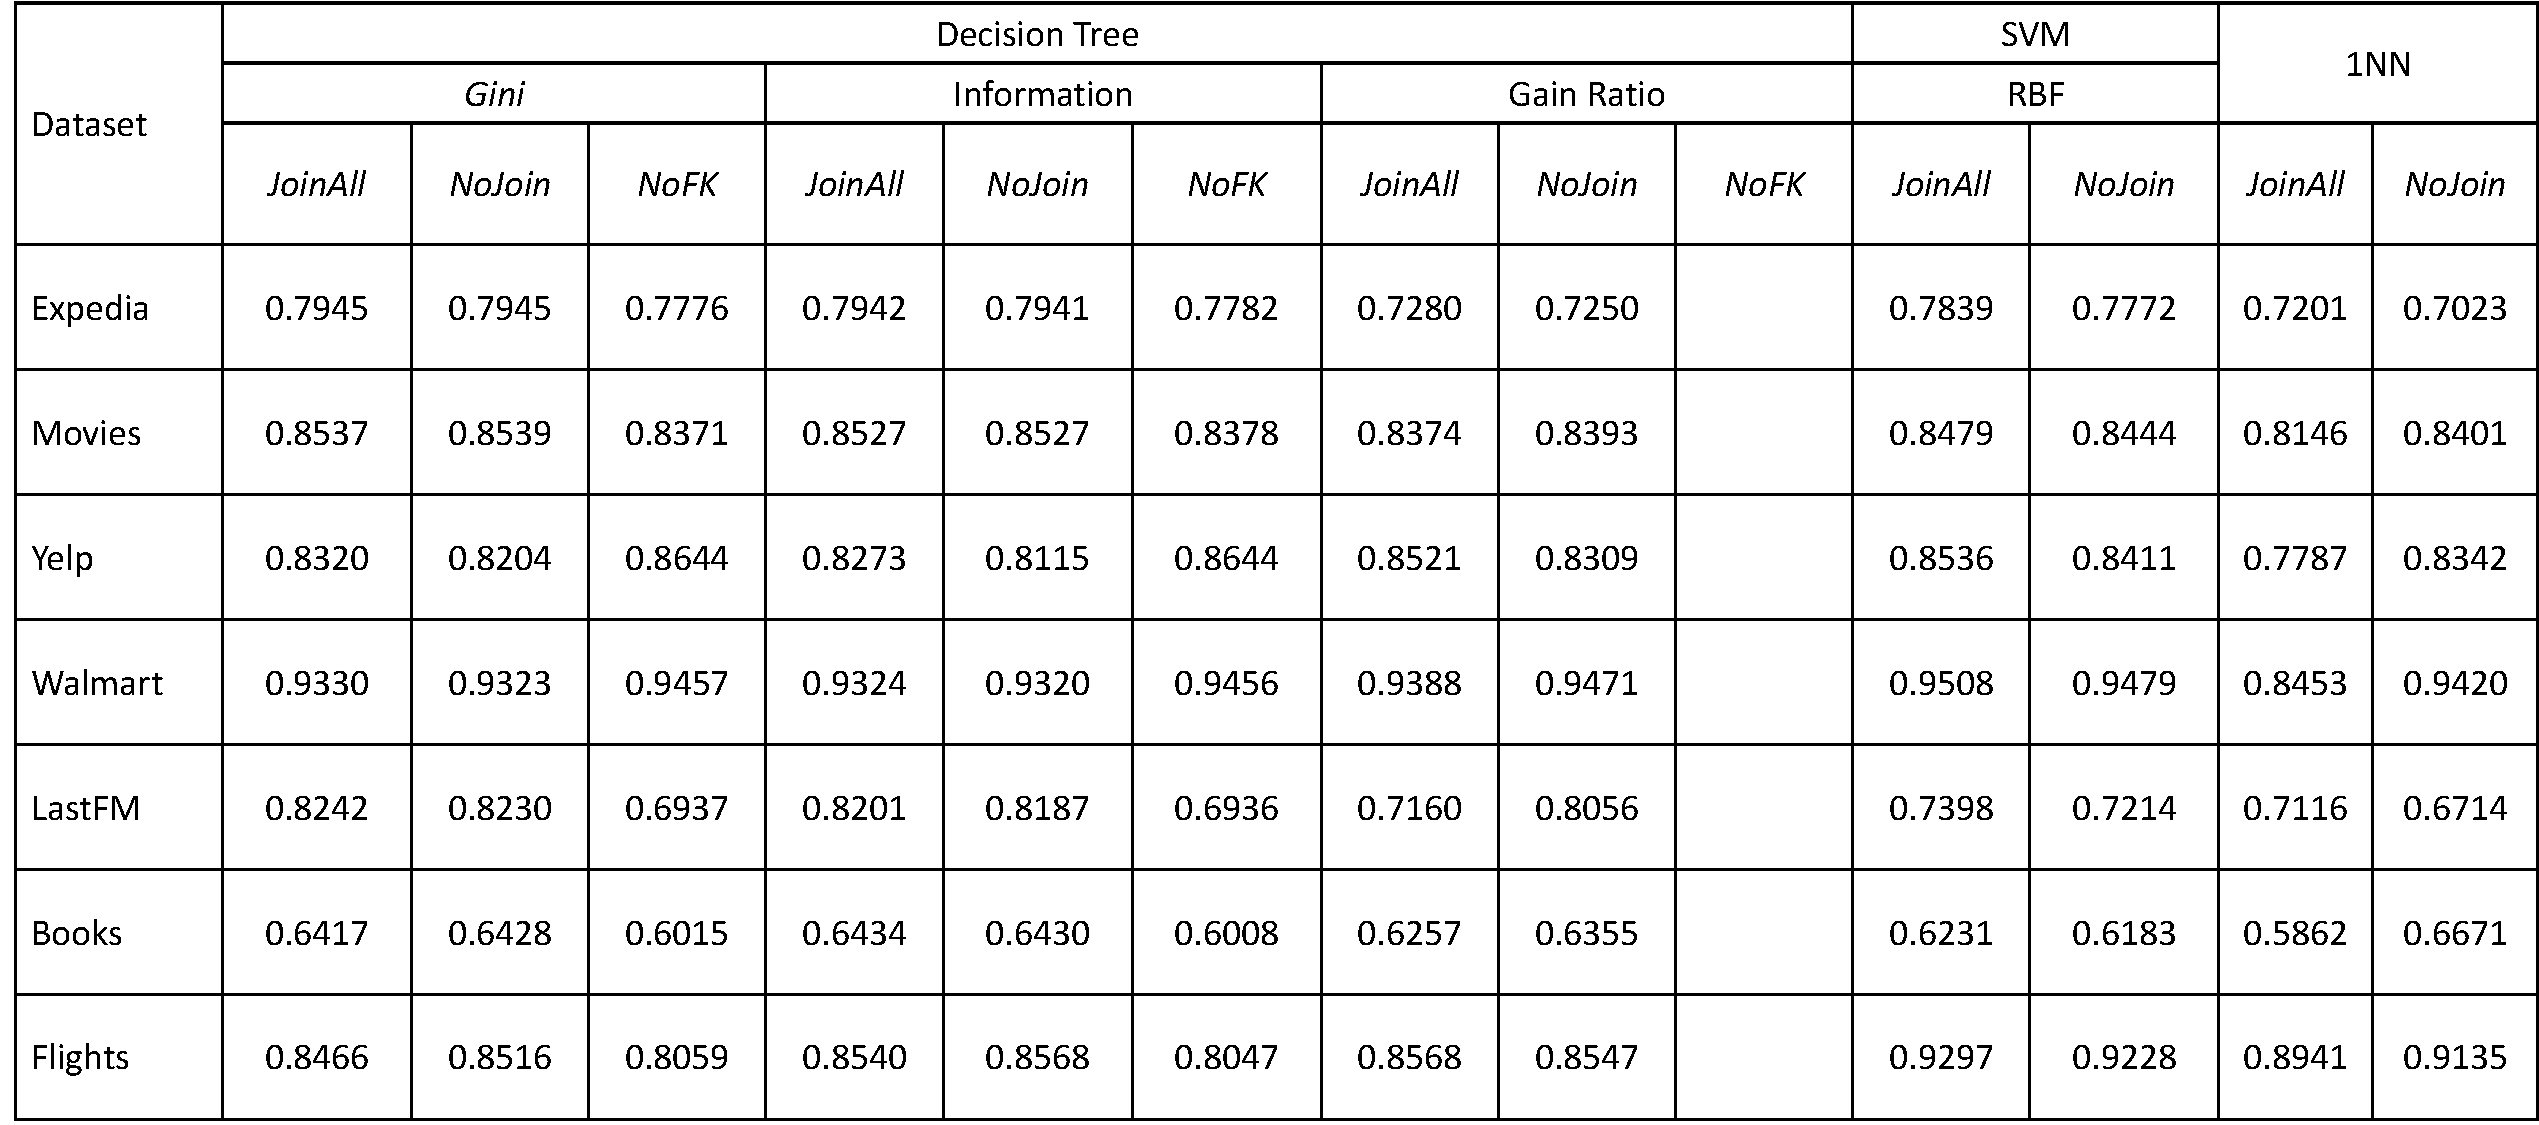
\includegraphics[width=0.99\linewidth]{table2.pdf}
\caption{Holdout test accuracy on the real-world datasets.}
\label{Table:RealTest}
\end{table*}

\textit{Walmart}: predict if department-wise sales will be high using past sales (fact table) joined with stores and weather/economic indicators (two dimension tables).
\textit{Flights}: predict if a route is codeshared by using other routes (fact table) joined with airlines, source, and destination airports (three dimension tables).
\textit{Yelp}: predict if a business will be rated highly using past ratings (fact table) joined with users and businesses (two dimension tables).
\textit{MovieLens}: predict if a movie will be rated highly using past ratings (fact table) joined with users and movies (two dimension tables).
\textit{Expedia}: predict if a hotel will be ranked highly using past search listings (fact table) joined with hotels and search events (two dimension tables but one foreign key has an 
``open'' domain, i.e., past values will not be seen in the future, and hence cannot be used).
\textit{LastFM}: predict if a song will be played often using past play level information (fact table) joined with users and artists (two dimension tables).
\textit{Books}: if a book will be rated highly using past ratings (fact table) joined with readers and books (two dimension tables).

\subsection{Methodology}
Each dataset comes pre-split 50\%:25\%:25\% for training-validation-test. We retain the splits as is.
We compare two approaches: \textit{JoinAll}, which joins all base tables to provide all features to the classifier (the current widespread practice), and \textit{NoJoin},
which avoids all foreign features a priori (the approach we study). We compare them for decision trees (CART), SVMs, and ANN. We also report results with the two 
linear models discussed in prior work~\cite{hamlet} for a quick comparison: Naive Bayes and Logistic Regression.
For the decision trees, we consider all three popular split criteria: Gini, information gain, and gain ratio.
For the SVMs, we consider three popular kernels: RBF, quadratic, and linear.
We use the popular R packages ``rpart'' for the decision tree\footnote{For the gain 
ratio, we used ``CORElearn'' package in R.} and ``e1071'' for the SVM.  For the ANN, we use the popular Python library Keras on top of TensorFlow.
For Naive Bayes, we use the code from~\cite{hamlet}, while for logistic regression with L1 regularization, we use the popular R package ``glmnet."
We use the validation set to perform hyper-parameter tuning using a standard grid search for each model as described in detail below. Note that 
for Naive Bayes, there is no hyper-parameter tuning, while for logistic regression, the package performs automatic tuning internally.

\vspace{2mm}
\noindent \textit{Decision Tree}: There are two hyper-parameters to tune: \textit{minsplit} and \textit{cp}. \textit{minsplit} is the number of observations that 
must exist in a node for a split to be attempted. Any split that does not improve the fit by a factor of \textit{cp} is pruned off. 
The grid is set as follows: \textit{minsplit} $\in \{ 1, 10, 100, 10^3\}$ and \textit{cp} $\in \{10^{-4}, 10^{-3}, 0.01, 0.1, 0\}$   

\vspace{2mm}
\noindent \textit{RBF-SVM}: There are two hyper-parameters to tune: \textit{C} and $\gamma$. \textit{C} controls the cost of misclassification, while $\gamma > 0$ controls the bandwidth in the Gaussian kernel (given two data points $x_i$ and $x_j$): $k(x_i,x_j) = \exp(-\gamma \cdot \lVert{x_i - x_j} \rVert ^2 )$.
The grid is set as follows: \textit{C} $\in \{10^{-1}, 1, 10, 100, 10^3\}$ and $\gamma \in \{10^{-4}, 10^{-3}, 0.01, 0.1, 1, 10\}$.\footnote{On 
\textit{Movies} and\textit{Expedia} alone, we perform one more fine tuning step with $\gamma \in \{2^{-7}, 2^{-6},2^{-5}, 2^{-4}, 2^{-3}, 2^{-2},2^{-1}, 1,2, 2^{2}, 2^{3}\}$ to improve accuracy.}

\vspace{2mm}
\noindent \textit{Quad-SVM} \textbf{TODO}

\vspace{2mm}
\noindent \textit{Lin-SVM} \textbf{TODO}

\vspace{2mm}
\noindent \textit{ANN}: The network architecture comprises of 2 hidden units with 256 and 64 neurons and rectified linear unit as an activation function. In order to allow penalties on layer parameters, we do $L_2$ norm regularization. We tune the regularization parameter with grid set as $\{ 10^{-4}, 10^{-3}, 10^{-2} \}$. We choose the popular adam's algorithm for stochastic optimization and tune the learning rate with grid set as $\{ 10^{-3}, 10^{-2}, 10^{-1} \}$. 

For additional insights, we also include a third approach for the decision tree: \textit{NoFK}, which is simply \textit{JoinAll} but with the foreign keys dropped a priori.
Table~\ref{Table:RealTest} presents the results.
%We present the final results in the table \ref{Table:NeuralNet}.

\begin{table}[t]
\centering
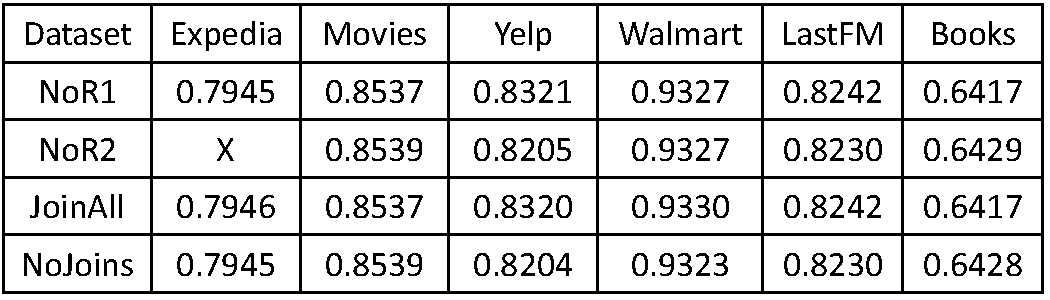
\includegraphics[width=\columnwidth,height=\textheight,keepaspectratio]{table4.pdf}
\begin{align*}
\textbf{Flights} : NoR1: 0.8466 \quad NoR2: 0.8490 \quad NoR3: 0.8483 \\
No R1,R2: 0.8488 \quad No R1,R3: 0.8481 \quad No R2,R3: 0.8519
\end{align*}
\caption{Robustness study for discarding dimension tables on the real-world datasets with a Gini decision tree.}
\label{Table:robustness}
\end{table}

\subsection{Results}

\subsubsection*{Accuracy}
Our first and most important observation is that for almost all the datasets (\textit{Yelp} being the exception) and for all three split criteria, the accuracy of the decision tree 
is comparable between \textit{JoinAll} and \textit{NoJoin}. The trend is virtually the same for the RBF-SVM and ANN as well! In stark contrast, 
the accuracy of \textit{NoJoin} is significantly worse than \textit{JoinAll} on more datasets with the linear models: linear SVM, logistic regression, and Naive Bayes.
Furthermore, for almost all datasets, \textit{NoFK} often has much lower accuracy than both \textit{JoinAll} and \textit{NoJoin}, which validates the importance 
of foreign key features.
Surprisingly, in some cases (e.g., Gini on \textit{Flights} and gain ratio on \textit{Books}), \textit{NoJoin} has even slightly higher accuracy than \textit{JoinAll}.
The only dataset for the decision tree on which \textit{NoJoin} has a gap of at least $0.01$ with \textit{JoinAll} and has lower accuracy is \textit{Yelp}. 
A similar behavior is seen on \textit{LastFM} and \textit{Books} as well for the SVM although the gap is smaller.
These results represent our key counter-intuitive finding: KFK joins are \textit{safer to avoid} with such high capacity classifiers than with the linear models!
Essentially, the extra overfitting caused by avoiding KFK joins is less pronounced with high capacity classifiers compared to linear models, which is rather surprising
because the VC dimension-based analysis in~\cite{hamlet} suggested the exact opposite.

To understand the accuracy results more deeply, we conduct a ``robustness'' experiment by discarding dimension tables one at a time instead of all at a time.
Table~\ref{Table:robustness} presents this experiment's results for the decision tree with Gini.
Discarding each dimension table one at a time (and also two at a time in the case of \textit{Flights}) did not differ much from \textit{NoJoin}, except for \textit{Yelp}.
On \textit{Yelp}, the accuracy drops only when $\textbf{R}_2$ (users table) is dropped. From Table~\ref{Table:datastats}, we find that the tuple ratio for $\textbf{R}_2$ in 
\textit{Yelp} is extremely low: $2.5$. So, there are not enough training examples per unique foreign key value for $\textbf{R}_2$ in \textit{Yelp}, i.e., its tuple ratio is too 
low.\footnote{Interestingly, the tuple ratio is similarly low ($2.6$) for $\textbf{R}_2$ in \textit{Books} but the error of \textit{NoJoin} is not much higher. So, the tuple 
ratio seems to be a \textit{conservative} indicator: it can tell if an error is likely to rise but the error may not actually rise in some case.}
Almost every other dimension table can safely be discarded. A similar situation arises for the SVM on \textit{Yelp}, as well as, \textit{LastFM}, and \textit{Books}. 

Overall, of the $14$ dimension tables across the $7$ datasets that can potentially be discarded, we are able to discard $13$ for the decision tree, with 
the tuple ratio threshold being about $3$x. For the SVM, we are able to discard $11$ of them, with the tuple ratio threshold being about $6$x.
These results are surprising given the more conservative behavior seen on linear models in~\cite{hamlet}. For example, for both Naive Bayes and logistic regression, only 
$7$ of the dimension tables could be discarded without affecting accuracy significantly, with the tuple ratio threshold being about $20$x. \textit{In other words, the decision tree
needs six times fewer training examples and the RBF-SVM needs three times fewer training examples than linear models to avoid extra overfitting when discarding foreign features}! 
This is counter-intuitive because conventional wisdom is that more complex ML models need more (not less) training examples to avoid extra overfitting.

For an interesting comparison that we will use later on, we also present the results for a classical ``braindead'' classifier: 1-nearest neighbor~\cite{mitchellbook} (from
package ``RWeka'' in R).
Surprisingly, as Table~\ref{Table:RealTest} shows,  its accuracy is sometimes comparable to decision trees and RBF-SVMs! 
More importantly, on most of the datasets, 1-NN with \textit{NoJoin} has a higher accuracy than with \textit{JoinAll}. We discuss this behavior further in Section 4.3.

\begin{table}[t]
\centering
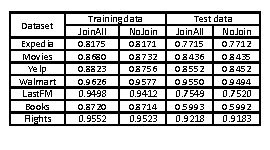
\includegraphics[width=\columnwidth,height=\textheight,keepaspectratio]{nn_table.pdf}
\caption{Accuracy on real-world datasets with ANN.}
\label{Table:NeuralNet}
\end{table}


\subsubsection*{Runtimes}

\textbf{TODO}

\begin{figure*}[t]
\centering
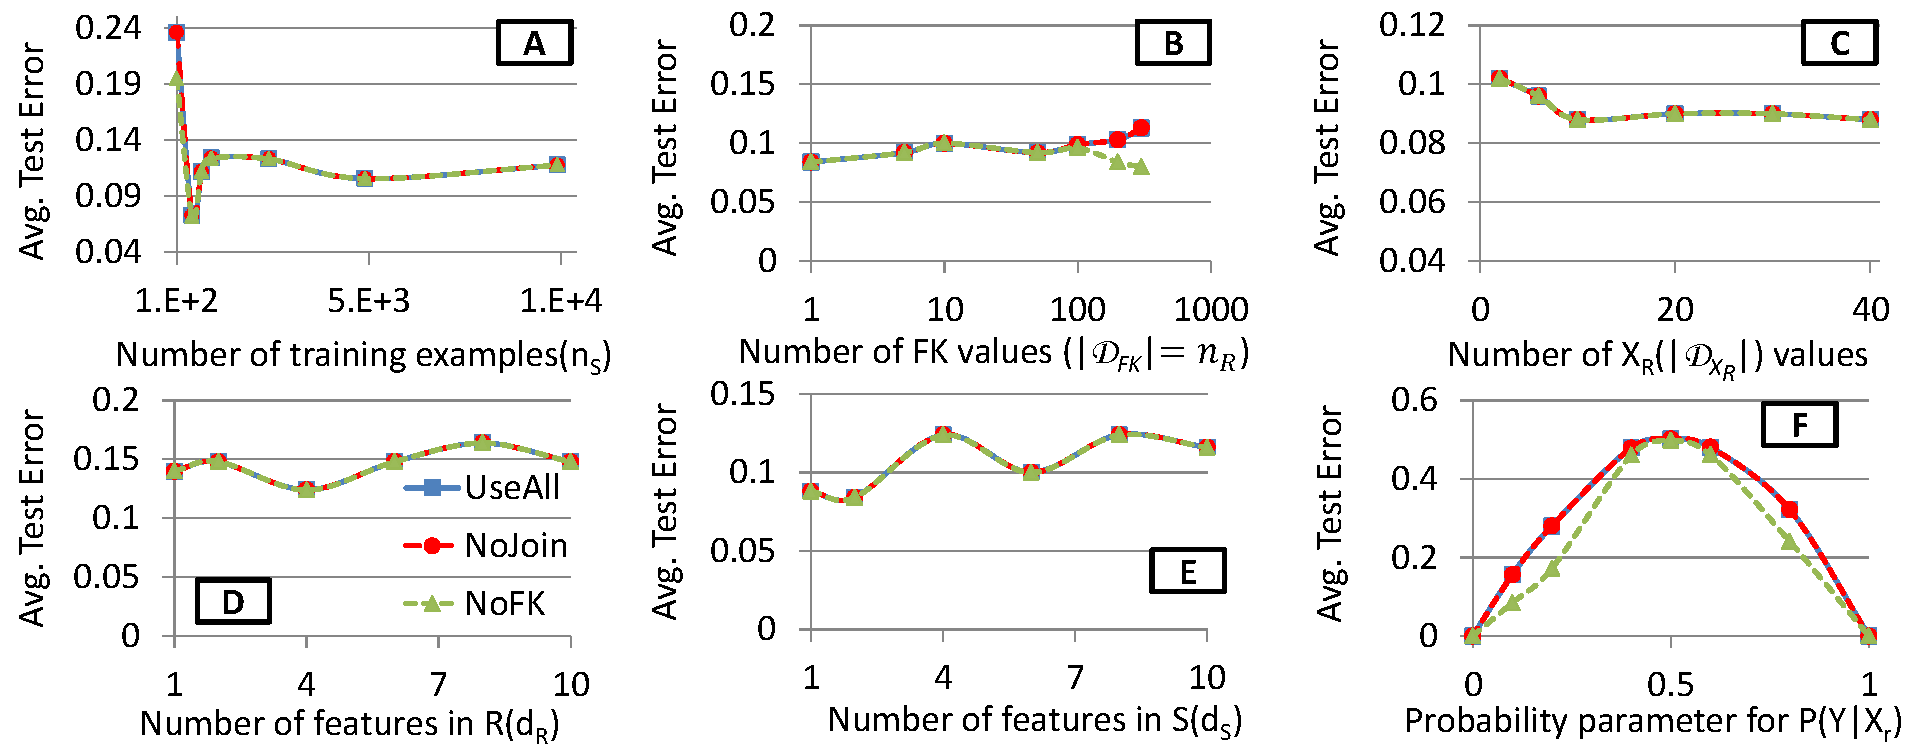
\includegraphics[width=0.85\linewidth]{onexr.pdf}
\caption{Simulation results for Scenario OneXr. For all plots except (E), we fix $p = 0.1$. Note that $n_R \equiv |\mathcal{D}_{FK}|$.
(A) Vary $n_S$, while fixing $(n_R, d_S, d_R) = (40, 4, 4)$.
(B) Vary $n_R$, while fixing $(n_S, d_S, d_R) = (1000, 4, 4)$.
(C) Vary $d_S$, while fixing $(n_S, n_R, d_R) = (1000, 40, 4)$.
(D) Vary $d_R$, while fixing $(n_R, d_S, d_R) = (1000, 40, 4)$.
(E) Vary $p$,  while fixing $(n_S, n_R, d_S, d_R) = (1000, 40, 4, 4)$.
(F) Vary $|\mathcal{D}_{X_r}|$, while fixing $(n_S, n_R, d_S, d_R) = (1000, 40, 4, 4)$; all other features in $\textbf{X}_R$ and $\textbf{X}_S$ are binary.
}
\label{Figure:OneXrSimulation}
\end{figure*}

\section{In-depth Simulation Study}	

We dive deeper into the behavior of the decision tree classifier using a simulation study in which we vary the properties of the 
underlying ``true'' data distribution. We focus on a two-table KFK join for simplicity. We sample datasets of different dimensions.
We use the decision tree for this study because it exhibited the maximum robustness to avoiding KFK joins on the real data. 
Our simulation study is designed to comprehensively ``stress test'' this robustness.
Note that our simulation methodology is not tied to decision trees; it is generic enough to be applicable to classifier because we only 
use standard generic notions of error and variance.

\paragraph*{Setup and Data Synthesis}
There is one dimension table \textbf{R} ($q=1$), and all of $\textbf{X}_S$, $\textbf{X}_R$, and $Y$ are boolean (domain size $2$).
We control the ``true'' distribution $P(Y,\textbf{X})$ and sample labeled examples in an IID manner from it.
We study two different scenarios for what features are used to (probabilistically) determine $Y$: \texttt{OneXr} and \texttt{XSXR}.
These scenarios represent opposite extremes for how likely the (test) error is likely to shoot up when $\textbf{X}_R$ is discarded
and $FK$ is used as a representative~\cite{hamlet}. In \texttt{OneXr}, a lone feature $X_r \in \textbf{X}_R$ determines $Y$; the 
rest of $\textbf{X}_R$ and $\textbf{X}_S$ are random noise (but note that $FK$ will not 
be noise because it functionally determines $X_r$). In \texttt{XSXR}, all features in $\textbf{X}_S$ and $\textbf{X}_R$ determine $Y$. 
Intuitively, \texttt{OneXr} is the worst-case scenario for discarding $\textbf{X}_R$ because $X_r$ is typically 
far more succinct than $FK$, which we expect to translate to less possibility of overfitting with NoJoin. Note that if we use $FK$ 
directly in $P$, $\textbf{X}_R$ can be more easily discarded because $FK$ conveys more information anyway; so, we skip this scenario.

The following data parameters are varied one at a time: number of training examples ($n_S$), size of foreign key domain ($|\mathcal{D}_{FK}|$ $=n_R$),
number of features in $\textbf{X}_R$ ($d_R$), and number of features in $\textbf{X}_S$ ($d_S$). We also sample $\frac{n_S}{4}$ examples each for the 
validation set (for hyper-parameter tuning) and the holdout test set (final indicator of error).
We generate $100$ different training datasets and measure the average test error and average net variance (as defined in~\cite{pedrobvd}) 
based on the different models obtained from these $100$ runs.

\subsection{Scenario OneXr}

The ``true'' distribution is set as follows: $P(Y=0|X_r=0)=P(Y=1|X_r=1)=p$, where $p$ is called the probability skew parameter that controls the Bayes error (noise).
The exact procedure for sampling examples is as follows: (1) Construct tuples of \textbf{R} by sampling $\textbf{X}_R$ values randomly (each feature value 
is an independent coin toss). (2) Construct the tuples of \textbf{S} by sampling $\textbf{X}_S$ values randomly (independent coin tosses). (3) Assign $FK$ 
values to \textbf{S} tuples uniformly randomly from $\mathcal{D}_{FK}$. (4) Assign $Y$ values to \textbf{S} tuples by looking up into their respective $X_r$ 
value (implicit join on $FK = RID$) and sampling from the above conditional distribution.

We compare the same three approaches: \textit{JoinAll}, which uses $\textbf{X} \equiv [\textbf{X}_S, FK, \textbf{X}_R]$, 
\textit{NoJoin}, which uses $\textbf{X} \equiv [\textbf{X}_S, FK]$ (i.e., discard $\textbf{X}_R$), and \textit{NoFK}, 
which uses $\textbf{X} \equiv [\textbf{X}_S, \textbf{X}_R]$ (i.e., discard $FK$).
% Our hypothesis is that \textit{JoinAll} and \textit{NoJoin} will exhibit similar errors in most cases. 
We include \textit{NoFK} for a lower bound on errors, since we know $FK$ does not determine determine $Y$ (although indirectly it 
does).\footnote{In general though, \textit{NoFK} could have much higher errors if $FK$ is part of the true distribution; indeed, \textit{NoFK} had 
much higher errors on many real datasets (Table~\ref{Table:RealTest}).}
Figure~\ref{Figure:OneXrSimulation} presents the results for the (holdout) test errors for varying each relevant data and distribution parameter, one at a time.

Interestingly, regardless of the parameter being varied, in almost all cases, \textit{NoJoin} and \textit{JoinAll} have virtually identical errors (close to the Bayes 
error)! From inspecting the actual decision trees learned in these two settings, we found that in almost all cases, $FK$ was used heavily for partitioning and seldom was 
a feature from $\textbf{X}_R$, including $X_r$, used. This suggests that $FK$ can indeed act as a good representative of $\textbf{X}_R$ even in this extreme sccenario. 
In contrast to these results,~\cite{hamlet} reported that for linear models, the errors of \textit{NoJoin} shot up compared to \textit{JoinAll} (a gap of nearly $0.05$)
as the tuple ratio starts falling below $20$. In stark contrast, as Figure~\ref{Figure:OneXrSimulation}(B) shows, even for a tuple ratio of just $3$, \textit{NoJoin} 
and \textit{JoinAll} have similar errors with the decision tree. This corroborates the results seen for the decision tree on the real datasets (Table~\ref{Table:RealTest}).
When $n_S$ becomes very low or when $|\mathcal{D}_{FK}|$ becomes very high, the absolute errors of \textit{JoinAll} and \textit{NoJoin} increase compared to \textit{NoFK}. 
This suggests that when the tuple ratio is very low, \textit{NoFK} is perhaps worth trying too. This is similar to the behavior seen on \textit{Yelp}. 
Overall, \textit{NoJoin} exhibits similar behavior as the current practice of \textit{JoinAll}.

Finally, we also ran this simulation scenario for the RBF-SVM (and 1-NN) and found the trends to be similar, except for the magnitude of the tuple ratio at which 
\textit{NoJoin} deviates from \textit{JoinAll}. Figure~\ref{Figure:OneXr1nnSVMSimulation} presents the results for the experiment in which we increase $|\mathcal{D}_{FK}|=n_R$, 
while fixing everything else, similar to Figure~\ref{Figure:OneXrSimulation}(B) for the decision tree. We see that for the RBF-SVM, the error deviation starts when the 
tuple ratio ($n_S/n_R$) falls below roughly $6$x. This corroborates the behavior seen for the decision tree on the real datasets (Table~\ref{Table:RealTest}).
The 1-NN, as expected, is far less stable and the deviation starts even at a tuple ratio of $100$x.


\begin{figure}[t]
\centering
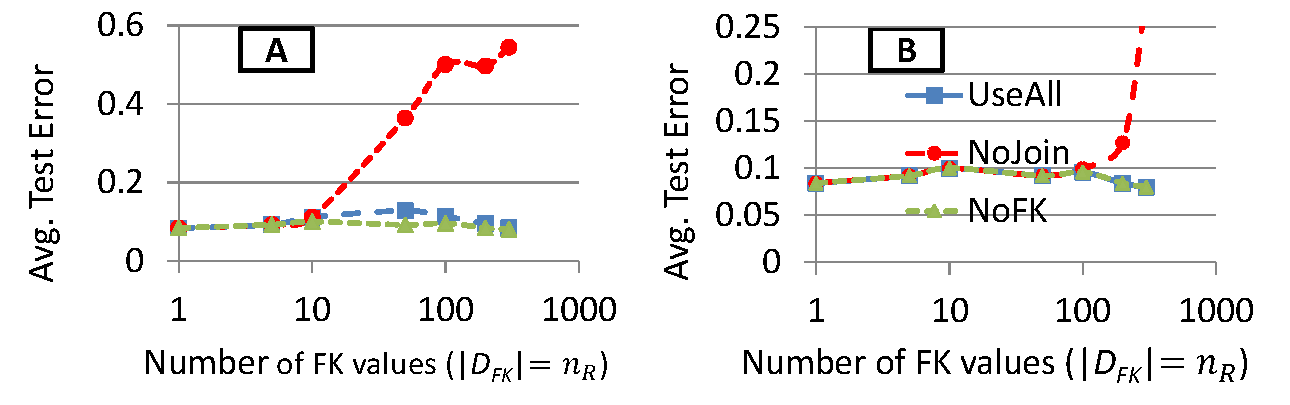
\includegraphics[width=0.99\linewidth]{onexr_svm_1nn.pdf}
\caption{Scenario OneXr simulations with the same setup as Figure~\ref{Figure:OneXrSimulation}(B), except for (A) 1-NN and (B) RBF-SVM.}
\label{Figure:OneXr1nnSVMSimulation}
\end{figure}

\begin{figure*}[t]
\centering
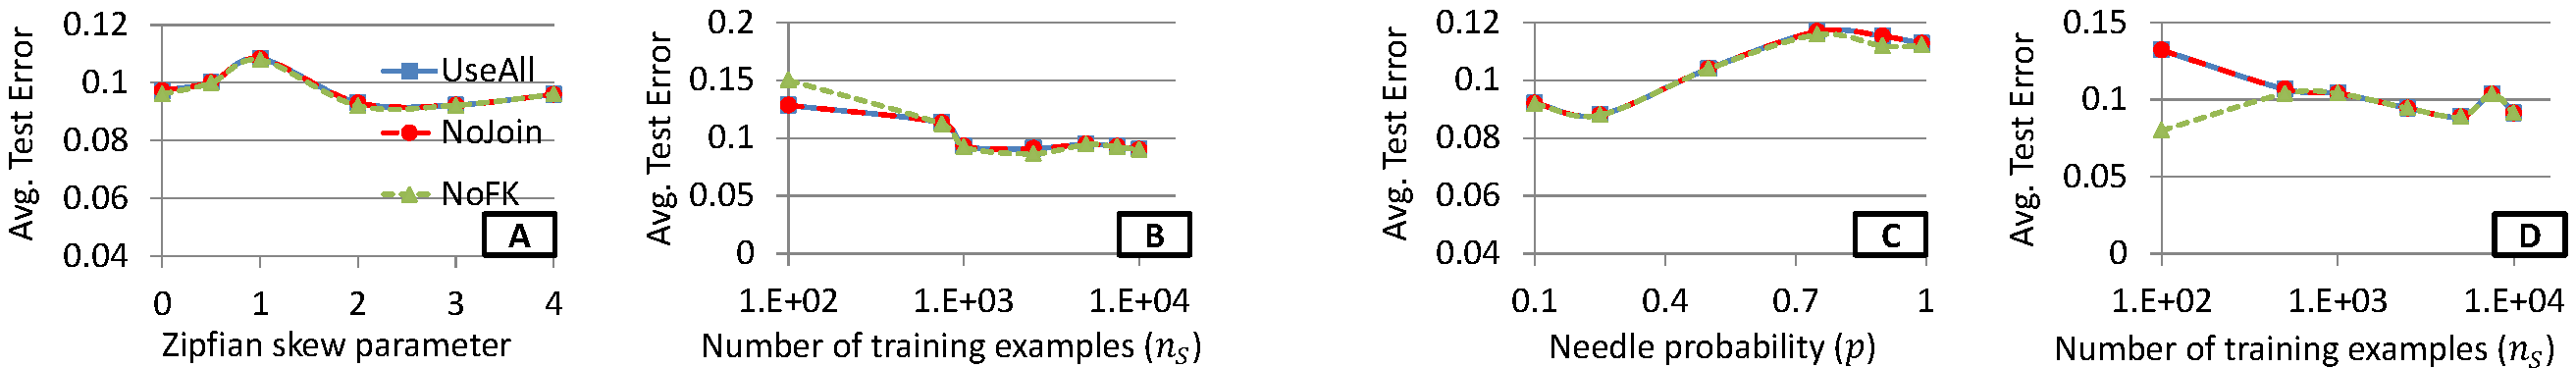
\includegraphics[width=2\columnwidth,height=\textheight,keepaspectratio]{skewfk_onexr.pdf}
\caption{Scenario \texttt{OneXr} simulations with skew in $P(FK)$. (A-B) Zipfian skew. (C-D) Needle-and-thread skew. For (A) and (C), we vary the respective skew parameter
(Zipfian skew parameter and needle probability), while fixing $(n_S, n_R, d_S, d_R) = (1000, 40, 4, 4)$. For (B) and (D), we vary $n_S$, while fixing $(n_R, d_S, d_R) = (40, 4, 4)$,
the Zipfian skew parameter to $2$ for (B), and the needle probability to $0.5$ for (D).
}
\label{Figure:OneXrZipfSimulation}
\end{figure*}

\paragraph*{Foreign Key Skew}
The regular \texttt{OneXr} scenario samples $FK$ uniformly randomly from $\mathcal{D}_{FK}$ (step 3 in the procedure). We now ask if a \textit{skew} in 
the distribution of $FK$ values could widen the gap between \textit{JoinAll} and \textit{NoJoin}. To study this scenario, we modify the data generation procedure slightly:
in step 3, we sample $FK$ values with a Zipfian skew or a needle-and-thread skew. The Zipfian skew simply uses a Zipfian distribution for $P(FK)$ controlled by the Zipfian
skew parameter. The needle-and-thread skew allocates a large probability mass (parameter $p$) to a single $FK$ value (the ``needle'') and uniformly distributes the rest of 
the probability mass to all other $FK$ values (the ``thread''). For the linear model case,~\cite{hamlet} reported that as the skew parameters increased, the gap widened.
Figure~\ref{Figure:OneXrZipfSimulation} presents the results for the decision tree.

Surprisingly, the gap between \textit{NoJoin} and \textit{JoinAll} does not widen significantly no matter how much skew introduced in either the Zipfian or the 
needle-and-thread case! This result further affirms the remarkable robustness of the decision tree when discarding foreign features. As expected, 
\textit{NoFK} is better when $n_S$ is low, while overall, \textit{NoJoin} is quite similar to \textit{JoinAll}.


\begin{figure*}[t]
\centering
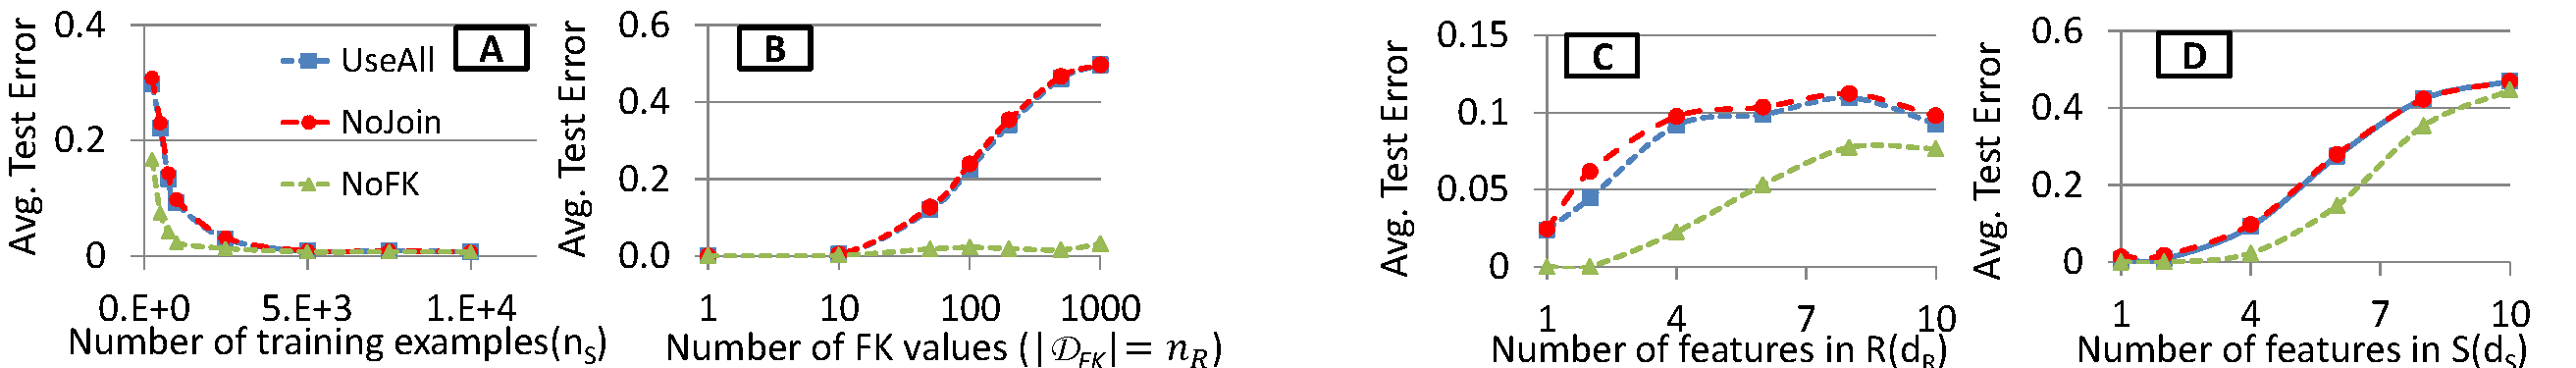
\includegraphics[width=0.99\linewidth]{xsxr1.pdf}
\caption{Simulation results for Scenario XSXR. The parameter values varied/fixed ($n_S$, $n_R$, $d_S$, and $d_R$) are the same as in Figure~\ref{Figure:OneXrSimulation} (A)-(D).}
\label{Figure:XsXrSimulation}
\end{figure*}

\subsection{Scenario XSXR}

Unlike the \textit{OneXr} scenario, we now create a true distribution that maps $\textbf{X} \equiv [\textbf{X}_S, \textbf{X}_R]$ to $Y$ without any Bayes error (noise).
The exact procedure for sampling examples is as follows: (1) Construct a true probability table (TPT) with entries for all possible values of 
$[\textbf{X}_S, \textbf{X}_R]$ and assign a random probability to each entry such that the total probability is $1$.
(2) For each entry in the TPT, pick a $Y$ value randomly and append the TPT entry; this ensures $H(Y|\textbf{X}) = 0$.
(3) Marginalize the TPT to obtain $P(\textbf{X}_R)$ and from it, sample $n_R = \mathcal{D}_{FK}$ tuples for \textbf{R} along with an associated sequential $RID$ value.
(4) In the original TPT, push the probability of each entry to $0$ if its $\textbf{X}_R$ values did not get picked for \textbf{R} in step 3.
(5) Renormalize the TPT so that the total probability is $1$ and sample $n_S$ examples ($Y$ values do not change) and construct \textbf{S}.
(6) For each tuple in \textbf{S}, pick its $FK$ value uniformly randomly from the subset of $RID$ values that map to its $\textbf{X}_R$ value in \textbf{R} (an implicit join).

We compare three settings: \textit{JoinAll}, \textit{NoJoin}, and \textit{NoFK}, with \textit{NoFK} meant to be a lower bound on the errors possible (because 
it uses the knowledge that $FK$ is not directly a part of the true distribution). Once again, our hypothesis is that \textit{JoinAll} and \textit{NoJoin} will exhibit similar 
errors in most cases, while \textit{NoFK} will perform better when the tuple ratio is low. Figure~\ref{Figure:XsXrSimulation} presents the results.

Once again, we see that \textit{NoJoin} and \textit{JoinAll} exhibit similar errors in almost all cases, with the largest gap being $0.017$ in Figure~\ref{Figure:XsXrSimulation}(C)).
Interestingly, even when the tuple ratio is close to $1$, the gap between \textit{NoJoin} and \textit{JoinAll} does not widen much. 
Figure~\ref{Figure:XsXrSimulation}(B)) shows that as $|\mathcal{D}_{FK}|$ increases, \textit{NoFK} remains at low overall errors, unlike both \textit{JoinAll} and \textit{NoJoin}.
But as we increase $d_R$ or $d_S$, the gap between \textit{JoinAll}/\textit{NoJoin} and \textit{NoFK} narrows because even \textit{NoFK} does not have enough training examples.
Of course, all gaps virtually disappear as the number of training examples increases, as shown by Figure~\ref{Figure:XsXrSimulation}(A).
Overall, \textit{NoJoin} exhibits similar behavior as the current practice of \textit{JoinAll} even in this scenario.

\begin{table*}
\centering
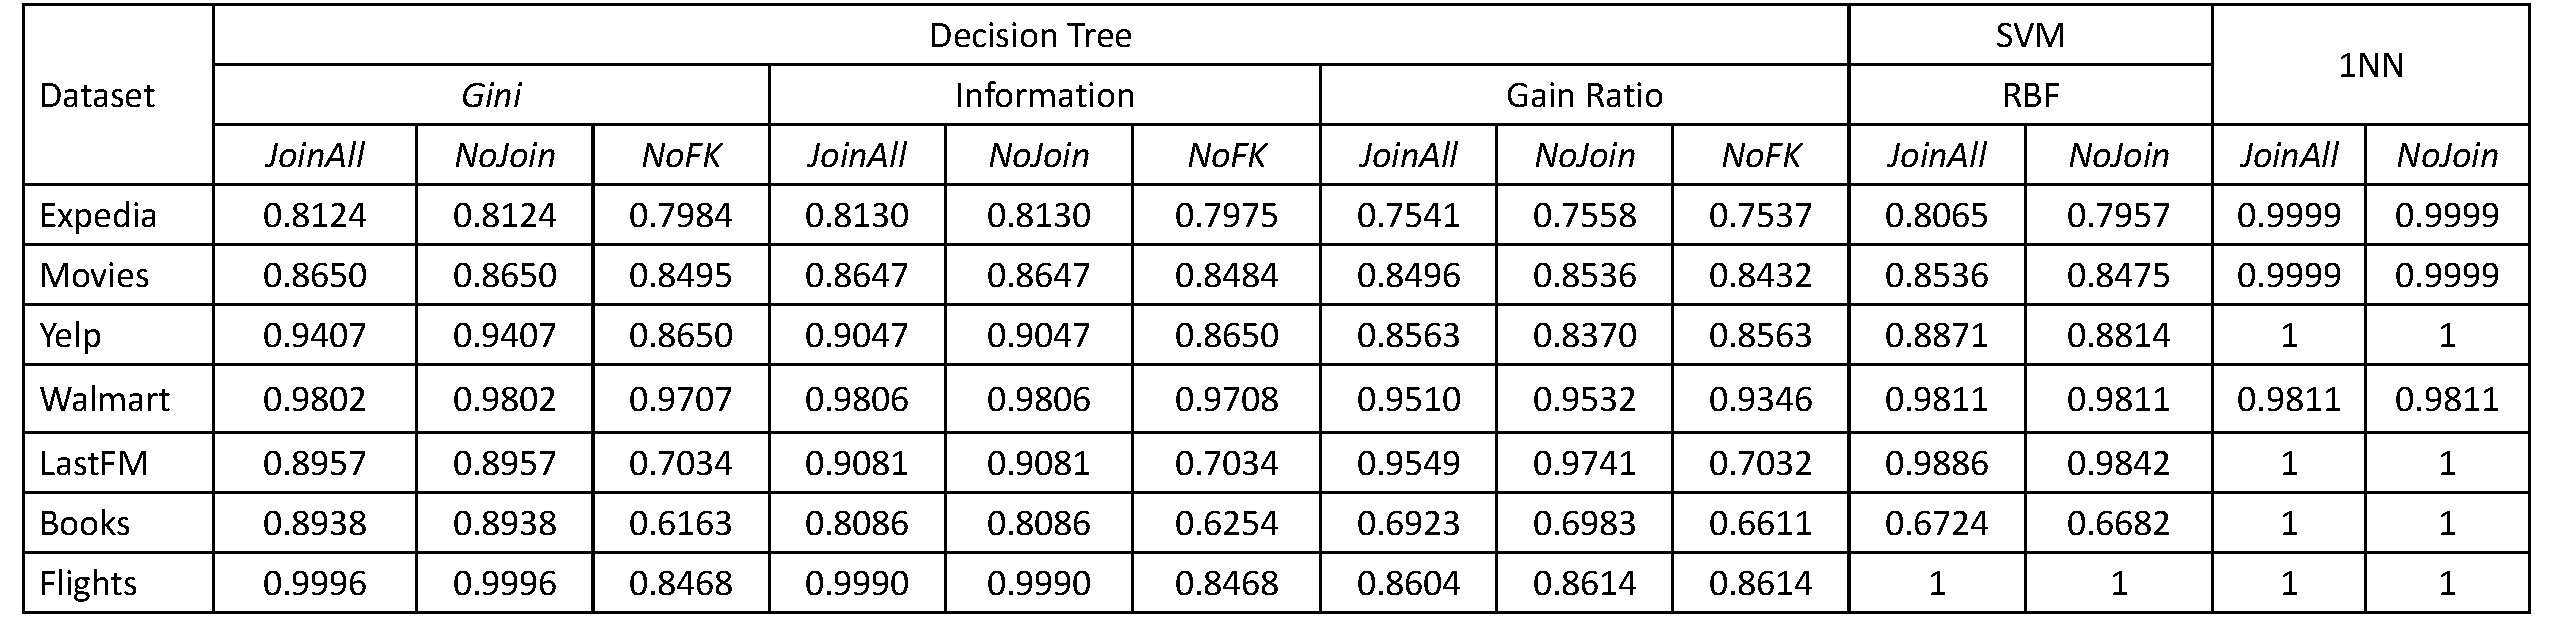
\includegraphics[width=2\columnwidth]{table3.pdf}
\caption{Training errors of the respective chosen models in the same experiment as Table~\ref{Table:RealTest}.}
\label{Table:RealTrain}
\end{table*}


\subsection{Scenario RepOneXr}
We now present results for a new simulation scenario in which the true distribution is precisely captured using a lone feature $X_r \in \textbf{X}_R$. We sample examples similarly as per the procedure mentioned earlier for OneXr, except that the tuples of $\textbf{R}$ will now be constructed by replicating the value of $X_r$ sampled for a tuple to create all the other features in $X_R$. That is, $X_R$ of an example is just the same value repeated $d_R$ times. Note that the FD $\textit{FK} \rightarrow X_R $ implies there are at least as many unique $FK$ values as $\textbf{X}_R$ values. Thus, by increasing the number of $FK$ values relative to $X_R$ values, we hope to increase the chance of the model getting ``confused'' with \textit{NoJoin}. Our goal is to see if this widens the gap between \textit{JoinAll} and \textit{NoJoin}.

\begin{figure}[h]
\centering
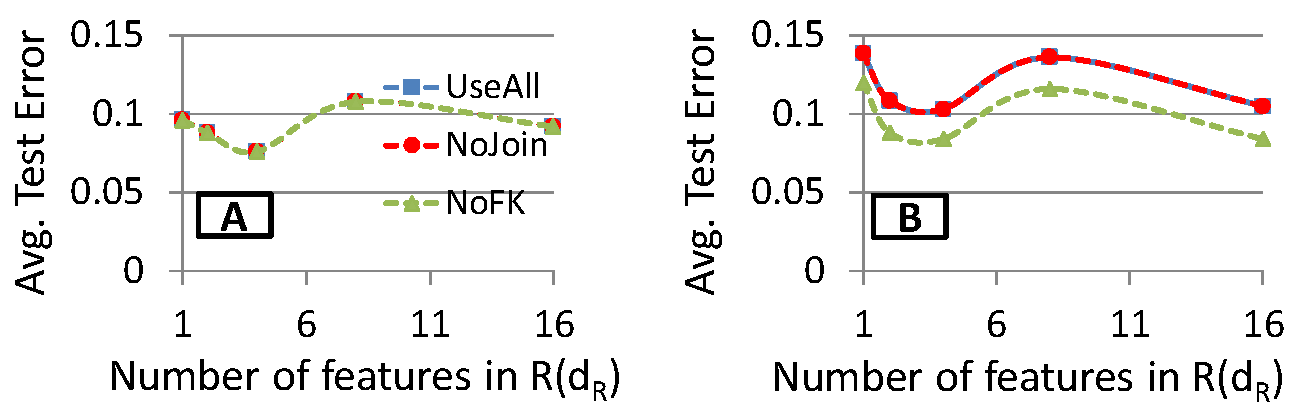
\includegraphics[width=0.99\linewidth]{onexr_jerrydt.pdf}
\caption{Scenario RepOneXr simulations for decision tree. (A) Vary $d_R$ while fixing $(n_S, n_R, d_S) = (1000, 40, 4)$. (B) Vary $d_R$ while fixing $(n_S, n_R, d_S) = (1000, 200, 4)$.}
\label{Figure:OneXrjerry_dt}
\end{figure}

Figure \ref{Figure:OneXrjerry_dt} presents the results for the two experiments on decision trees where (A) maintains a high tuple ratio of 25x and (B) maintains a low tuple ratio of 5x. Once again, \textit{JoinAll} and \textit{NoJoin} exhibit similar errors in both the cases. Finally, we run this simulation scenario for both RBF-SVM (shown in Figure \ref{Figure:OneXrjerry_svm}) and 1-NN (shown in Figure \ref{Figure:OneXrjerry_1nn}). We found the trends to be similar as section 4.1. We see that for RBF-SVM, the error deviation happens at a tuple ratio of 5x. The 1-NN, as expected is less stable and the deviation happens even at a higher tuple ratio of 25x. With low tuple ratios, the absolute errors of \textit{JoinAll} and \textit{NoJoin} increases compared to \textit{NoFK} for all the cases as we note in Figure \ref{Figure:OneXrjerry_dt},\ref{Figure:OneXrjerry_svm},\ref{Figure:OneXrjerry_1nn} (B).

\begin{figure}[h]
\centering
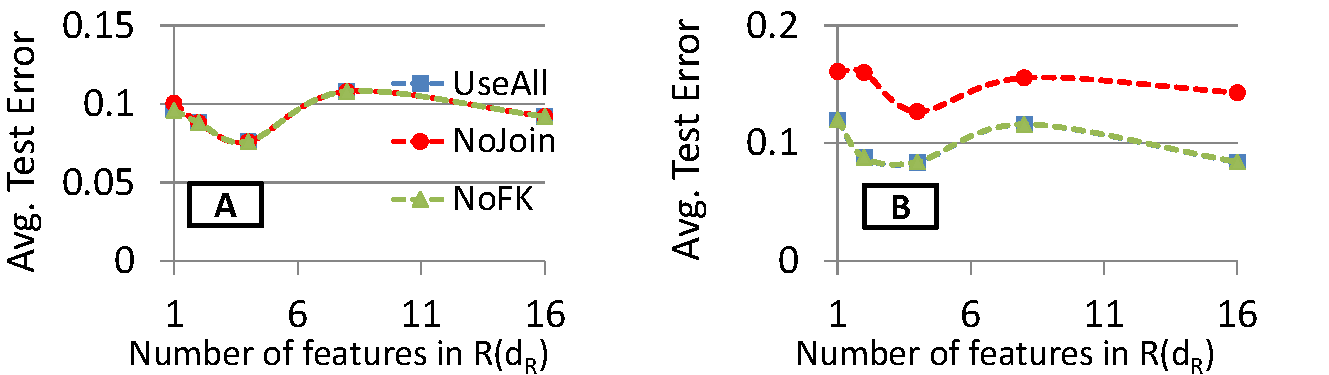
\includegraphics[width=0.99\linewidth]{onexr_jerrysvm.pdf}
\caption{Scenario OneXr simulations with same setup as Figure~\ref{Figure:OneXrjerry_dt}, except for SVM.}
\label{Figure:OneXrjerry_svm}
\end{figure}

\begin{figure}[h]
\centering
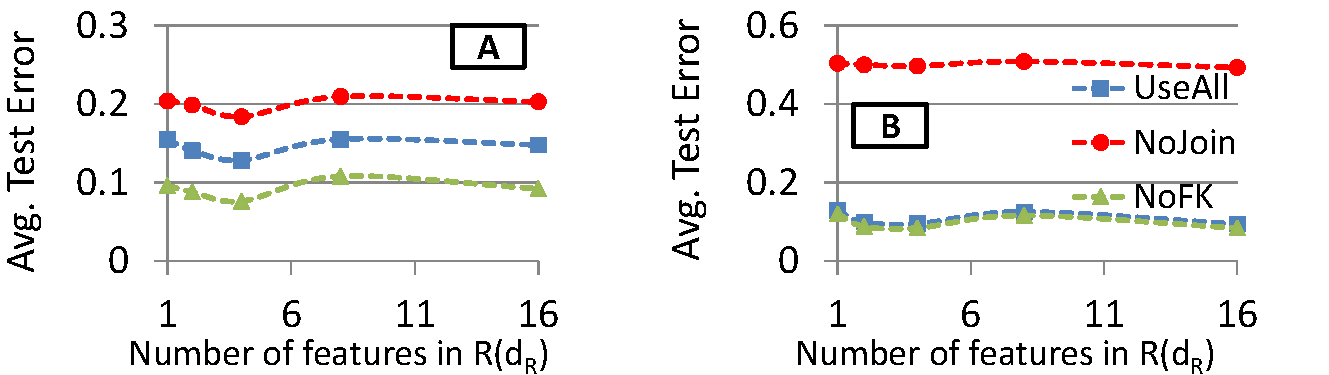
\includegraphics[width=0.99\linewidth]{onexr_jerry1nn.pdf}
\caption{Scenario OneXr simulations with same setup as Figure~\ref{Figure:OneXrjerry_dt}, except for 1-NN.}
\label{Figure:OneXrjerry_1nn}
\end{figure}


\section{Explanation and Open Theoretical Questions}

We now intuitively explain the surprising behavior of decision trees and RBF-SVM with \textit{NoJoin} vis-a-vis \textit{JoinAll}.
We first ask: {Does \textit{NoJoin} compromise the ``generalization error''?} The generalization error is the difference of the test and train errors.
Table~\ref{Table:RealTest} already provided the test accuracy. Table~\ref{Table:RealTrain} now provides the train accuracy. Clearly, \textit{JoinAll} vs 
\textit{NoJoin} are almost indistinguishable for the decision tree! The only exception is \textit{Yelp}, which we already noted. 
Note that the absolute generalization error is often high, which is expected for decision trees~\cite{dtreebias2}. 
For example, the train accuracy is nearly $100\%$ on \textit{Flights}, while the test accuracy on it is only $85\%$.
But the absolute generalization error is orthogonal to our focus; we only note that \textit{NoJoin} does not increase this difference significantly.
\textit{In other words, discarding foreign features did not significantly affect the generalization error of the decision tree!} 
The generalization errors of the RBF-SVM also exhibit a similar trend.

Returning to 1-NN, Table~\ref{Table:RealTest} showed that it has similar accuracy as the RBF-SVM on some datasets. We now explain why that comparison is useful: the RBF-SVM 
essentially behaves similar to the 1-NN in some cases when $FK$ is used (both \textit{JoinAll} and \textit{NoJoin})! But this is not necessarily ``bad'' for its test accuracy.
Note that $FK$ is represented using the standard one-hot encoding for RBF-SVM and 1-NN. So, $FK$ can contribute to a maximum distance of $2$ in a (squared) Euclidean distance between 
two examples $x_i$ and $x_j$.
But since $\textbf{X}_R$ is functionally dependent on $FK$, if $x_i.FK = x_j.FK$, then $x_i.\textbf{X}_R = x_j.\textbf{X}_R$. So, if $x_i.FK = x_j.FK$, the only contributor to 
the distance is $\textbf{X}_S$. But in many of the datasets, since $\textbf{X}_S$ is empty ($d_S = 0$), $FK$ becomes the sole determiner of the distances for \textit{NoJoin}.
This is akin to sheer \textit{memorization} of a feature's large domain. Since we operate on features with finite domains, test examples will also have $FK$ from that domain. 
Thus, memorizing $FK$ does not hurt generalization. While this seems similar to how deep neural networks excel at sheer memorization but still offer good test accuracy~\cite{rechtdnn}, 
the models in our setting are not necessarily memorizing all features -- only the foreign keys.
A similar explanation holds for the decision tree. If $\textbf{X}_S$ is not empty, then it will likely play a major role in the distance computations and our setting 
becomes more similar to the traditional single-table learning setting (no FDs).

We now explain why \textit{NoJoin} might deviate from \textit{JoinAll} when the tuple ratio is very low for the RBF-SVM. Even if $x_i.FK \ne x_j.FK$, it is possible that 
$x_i.\textbf{X}_R = x_j.\textbf{X}_R$. Suppose the ``true'' distribution is captured by $\textbf{X}_R$, e.g., as in OneXr. 
If the tuple ratio is very low, there are many $FK$ values but the number of $\textbf{X}_R$ values might still be small. In this case, given $x_i$, RBF-SVM (and 1-NN) is more 
likely to pick an $x_j$ that minimizes the distances on $\textbf{X}_R$, thus potentially yielding lower errors. But since \textit{NoJoin} does not have access to 
$\textbf{X}_R$, it can only use $\textbf{X}_S$ and $FK$. So, if $\textbf{X}_S$ is mostly noise, the possibility of the model getting ``confused'' 
increases. To see why, if there are very few other examples that share $x_i.FK$, then matching on $\textbf{X}_S$ might become more important. 
Thus, a non-match on $FK$ becomes more likely, which means a non-match on the implicit $\textbf{X}_R$ becomes more likely, which in turns makes higher errors more likely. 
But if there are more examples that share $x_i.FK$, then a match on $FK$ is more likely. Thus, as the tuple ratio increases, the gap between \textit{NoJoin} 
and \textit{JoinAll} disappears, as Figure~\ref{Figure:OneXr1nnSVMSimulation} showed. Internally, the RBF-SVM seems more robust to such chance mismatches by learning a higher-level 
relationship between all features compared to the stark 1-NN. Thus, the RBF-SVM is more robust to discarding foreign features at lower tuples ratios than 1-NN.

Finally, focusing on the decision tree, its internal feature selection and partitioning seems to make it quite robust to noise from any other features. Suppose again the ``true'' 
distribution is similar to OneXr. Since $FK$ already encodes all information that $\textbf{X}_R$ provides~\cite{hamlet}, the tree almost always uses $FK$ in its partitioning, 
often multiple times. This is not necessarily ``bad'' for test accuracy because test examples share the $FK$ domain. 
But when the tuple ratio becomes extremely low, the chance of $\textbf{X}_S$ ``confusing'' the tree over the information $FK$ provides goes up, potentially 
leading to higher errors with \textit{NoJoin}. \textit{JoinAll} escapes such a confusion thanks to $\textbf{X}_R$. If $\textbf{X}_S$ is empty, then $FK$ will almost surely
be used for partitioning. But with very few training examples per $FK$ value, the chance of sending it to a wrong partition goes up, leading to higher errors. It turns out 
that even with just $3$ or $4$ training examples per $FK$ value, such issues get mitigated. Thus, the decision tree seems even more robust to discarding foreign features.

\eat{
\begin{figure}[t]
\centering
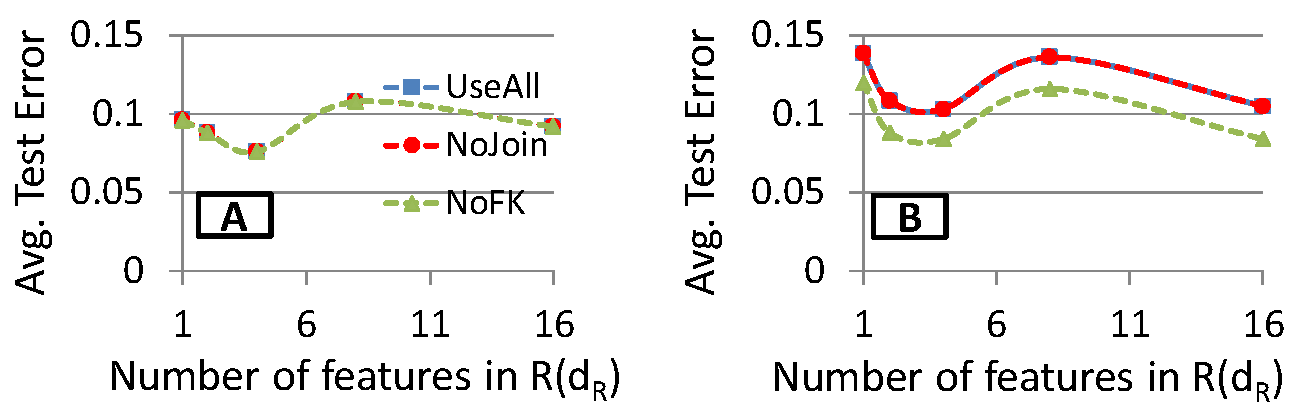
\includegraphics[width=\columnwidth,height=\textheight,keepaspectratio]{onexr_jerrydt.pdf}
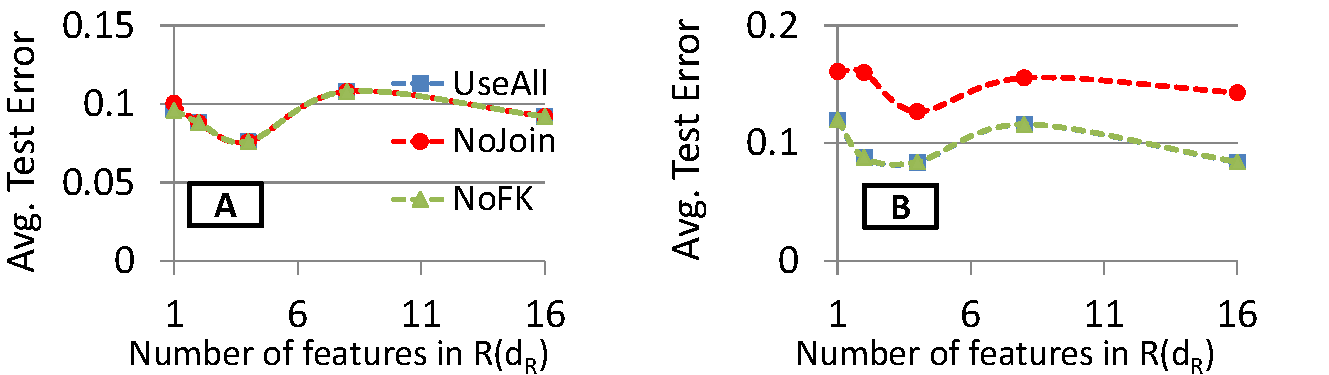
\includegraphics[width=\columnwidth,height=\textheight,keepaspectratio]{onexr_jerrysvm.pdf}
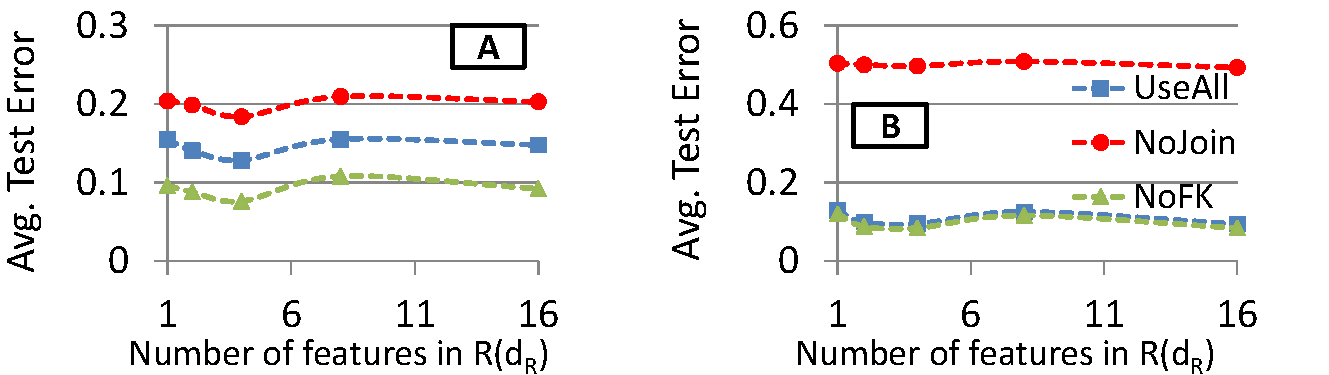
\includegraphics[width=\columnwidth,height=\textheight,keepaspectratio]{onexr_jerry1nn.pdf}
\caption{OneXr simulation for repeated Xr Features}
\label{Figure:OneXrjerry}
\end{figure}

\paragraph*{Scenario RepeatedOneXr}
}

While our intuitive explanations capture the fine-grained behavior of the decision tree and RBF-SVM with \textit{NoJoin} vis-a-vis \textit{JoinAll}, there are clearly many 
open questions for deeper ML theoretical research. Is it possible to quantify the probability of wrong partitioning with a decision tree as a function of the properties of 
the data? Is it possible to quantify the probability of mismatched examples being picked for the RBF-SVM as a similar function? Why does the theory of VC-dimensions predict 
the opposite of the observed behavior with these models? How do we quantify their generalizability if memorization is allowable and what forms of memorization are allowable?
Answering these questions would provide deeper insights into the effects of KFKDs and FDs on the generalizability and accuracy of such classifiers. It could also yield more 
formal mechanisms to characterize when discarding foreign features is feasible beyond just looking at tuple ratios.

\textbf{TODO: conditional FDs; partial avoidance; interaction with MVDs, EMVDs, JDs?}

\section{Making FK Features Practical}

We now discuss two key practical issues caused by the large domains of foreign key features and explore how standard approaches can be used to resolve them. 
In contrast to prior work on handling regular large-domain features~\cite{dtreebias1}, foreign key features are distinct in that they have coarser-grained 
side information available in the foreign features, which can be exploited, if possible.

\subsection{Foreign Key Domain Compression}

While foreign keys often act as good representatives of foreign features for \textit{accuracy},
they pose a practical bottleneck for \textit{interpretability} due to their domain sizes.
For example, it is hard to visualize a decision tree that uses a foreign key feature with 1000s of values.
In order to make foreign key features more practical, we consider a simple approach that is standard in the ML literature:
\textit{lossy domain compression} to a (much) smaller user-defined domain size. Essentially, given a 
foreign key feature $FK$ with domain $\mathcal{D}_{FK}$ recoded as $[m]$ (where $m = |\mathcal{D}_{FK}|$) and a user-specified 
positive integer ``budget'' $l \ll m$, we want a mapping $f: [m] \rightarrow [l]$.

\begin{figure}[t]
\centering
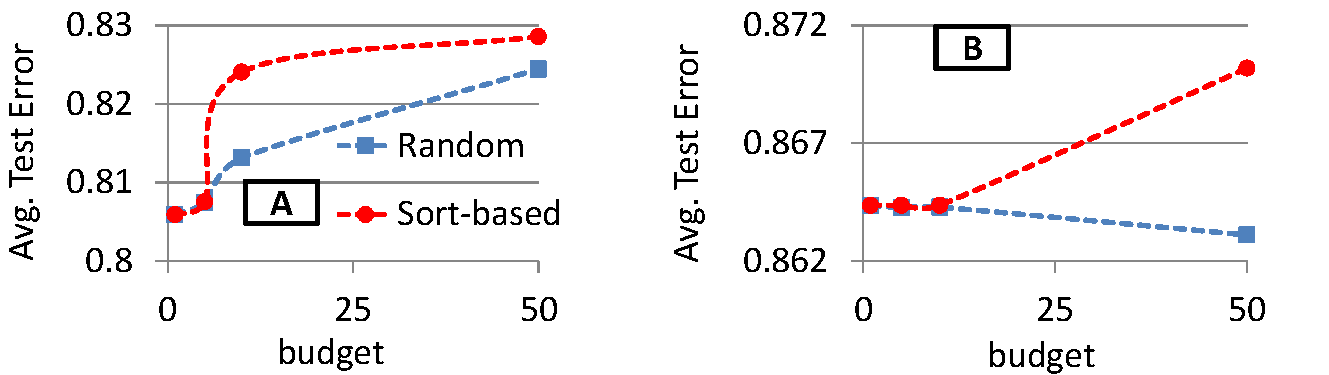
\includegraphics[width=0.99\linewidth]{dom_comp.pdf}
\caption{Domain compression. (A) \textit{Flights}. (B) \textit{Yelp}.}
\label{Figure:Compression}
\end{figure}

A standard unsupervised method to construct $f$ is the \textit{Random hashing} trick~\cite{hashingtrick}, i.e., randomly hash from $[m]$ to $[l]$.
We also try a simple supervised method we call the \textit{Sort-based} method to preserve more of the information contained 
in $FK$ about $Y$. Sort-based is a greedy approach: sort $\mathcal{D}_{FK}$ based on $H(Y|FK=z), ~z \in \mathcal{D}_{FK}$, compute the 
differences among adjacent pairs of values, and pick the boundaries corresponding to the top $l-1$ differences (ties broken randomly). 
This gives us an $l$-partition of $\mathcal{D}_{FK}$. The intuition is that by grouping $FK$ values that have comparable conditional entropy, 
$H(Y|f(FK))$ is unlikely to be much higher than $H(Y|FK)$. Note that the lower $H(Y|FK)$ is, the more informative $FK$ is to predict $Y$. 
We leave more sophisticated approaches to future work.

We now empirically compare the above two heuristics using two of the real datasets for the Gini decision tree with \textit{NoJoin}. Our methodology 
is as follows. We retain the 50:25:25 train-validate-test split from before. We use the training split to construct $f$ and then compress $FK$ for 
the whole dataset. We then use the validation set as before to tune the hyper-parameters and measure the holdout test error. For random hashing, we 
report the average across five runs. Figure~\ref{Figure:Compression} presents the results.

On \textit{Yelp}, both \textit{Random} and \textit{Sort-based} have comparable accuracy although Sort-based is marginally higher, especially
as the budget $l$ increases. But on \textit{Flights}, we see a larger gap for some values of $l$ although the gap narrows as the $l$ increases.
The test accuracy with the whole $\mathcal{D}_{FK}$ ($l=m$) for \textit{NoJoin} on \textit{Flights} was $0.8516$ (see Table~\ref{Table:RealTest}). So, 
it is surprising the test accuracy is about $0.83$ with such high compression. Even more surprisingly, the test accuracy with the whole 
$\mathcal{D}_{FK}$ ($l=m$) for \textit{NoJoin} on \textit{Yelp} was $0.8204$ and for \textit{NoFK} was $0.8644$. So, with domain compression,
we see significantly higher accuracy for \textit{NoJoin}, even higher than \textit{NoFK}! Overall, these results suggest that $FK$ domain compression 
is a promising way to resolve the large-domain issue rather than simply dropping $FK$.

\eat{
Thus, to make foreign key features more practical, we consider a simple approach: \textit{compress} their domains to a (much) smaller 
user-defined domain size. This is inspired by the hashing trick~\cite{hashingtrick} but instead of an unsupervised random 
compression, we propose a deterministic supervised compression that optimizes some criterion related to accuracy. A key benefit of 
this approach is potentially higher accuracy, while obtaining an interpretable grouping of domain values.
We consider a natural criterion for maximization: \textit{mutual information} of the compressed foreign key with the target.

Formally, given the target $Y$ with domain $\mathcal{D}_Y$, a foreign key feature $FK$ with domain $\mathcal{D}_{FK}$ recoded as $[m]$ 
(where $m = |\mathcal{D}_{FK}|$) and a positive integer ``budget'' $l \ll m$, obtain a mapping $f: [m] \rightarrow [l]$ such that $I(Y; f(FK))$ is maximized,
or equivalently, $H(Y|f(FK))$ is minimized. Essentially, this is a partitioning problem in which we $\mathcal{D}_{FK}$ is partitioned into $l$ subsets. 
We reformulate this as a $0/1$-optimization problem over an $m \times l$ indicator variable matrix $v$.
The input constants are $|\mathcal{D}_Y| \cdot l$ frequency counts of the joint $(Y, FK)$ values in the training dataset, denoted $c_{y, x}$.
The problem then becomes the following:

\begin{equation*}
\begin{aligned}
& \underset{v}{\text{min}}
& & \sum_{y \in \mathcal{D}_Y} \sum_{j=1}^l \bigg(\sum_{i=i}^m c_{y,i} \cdot v_{i,j} \bigg) log \bigg(\frac{\sum_{y' \in \mathcal{D}_Y} \sum_{i=i}^m c_{y,i} \cdot v_{i,j}}{\sum_{i=i}^m c_{y,i} \cdot v_{i,j}}\bigg) \\
& \text{s.t.}
& & \sum_{j=1}^l v_{i,j} = 1, \; i = 1, \ldots, m
\end{aligned}
\end{equation*}

The optimization problem is non-convex and hard to optimize in a brute-force  way due to the number of variables (potentially millions). Thus, we propose two heuristics: \textit{SortBased} and \textit{TreeBased}.

\textit{SortBased} is a greedy approach in which we sort $\mathcal{D}_{FK}$ based on $H(Y|FK=z), ~z \in \mathcal{D}_{FK}$, compute the differences among adjacent pairs of values, and pick the boundaries corresponding to the top $l-1$ differences (ties broken randomly). This gives us an $l$-partition of $\mathcal{D}_{FK}$. The intuition is that by grouping $FK$ values that have comparable conditional entropy values, $H(Y|f(FK))$ is unlikely to increase much compared to $H(Y|FK)$. This approach operates on the training split.

\textit{TreeBased} is a post-hoc approach in which we first learn a decision tree that includes $FK$. Internally, the tree induces a partitioning of 
$\mathcal{D}_{FK}$. We simply construct $f$ using this partitioning information. Let $r$ be the number of subsets of $\mathcal{D}_{FK}$ at the lowest levels of the tree 
(finest-grained partitioning). If $r = l$, each subset directly corresponds to a value in $[l]$. If $r > l$, we use the same greedy approach used for the SortBased 
approach to merge the subsets until we end up with $l$ subsets. Finally, if $r < l$, we simply leave the partitioning as is because we already satisfy the user's budget;
the co-domain of $f$ is then only $[r]$ instead of $[l]$. This approach utilizes both the training and validation splits for learning the best decision tree that includes $FK$, with .

We now empirically compare the accuracy of the above two heuristics against random hashing as a baseline with $l$ as the number of buckets. 
We use the real-world datasets for this experiment and our methodology is as follows. We retain the 50:25:25 train-validate-test split.
\textit{SortBased} and random hashing use just the training split to construct $f$ and then compress $FK$ for the whole dataset. We then use
the validation set as before to tune the hyper-parameters and measure the holdout test error. For random hashing, we report the average across 
five runs. For \textit{TreeBased}, we first learn a decision tree using the original training and validation sets, construct $f$ and compress 
$FK$ for the whole dataset, and then measure the holdout test error.
}


\subsection{Foreign Key Smoothing}

Another issue caused by large $|\mathcal{D}_{FK}|$ is that some $FK$ values might not arise in the train set but arise 
in the test set or during deployment. This is not a cold start issue -- the $FK$ values are all still from the fully known $\mathcal{D}_{FK}$. 
This issue arises because there are not enough labeled examples to cover all of $\mathcal{D}_{FK}$ during training. 
Typically, this issue is handled using some form of \textit{smoothing}, e.g., Laplacian smoothing
for Naive Bayes by adding a pseudocount of $1$ to all frequency counts~\cite{mitchellbook}.
While similar smoothing techniques have been studied for probability estimation using decision trees~\cite{pedro2003}, to the best of our knowledge, 
this issue has not been handled in general for classification using decision trees. In fact, popular decision tree implementations in R simply 
crash if a value of $FK$ not seen during training arises during testing! Note that SVMs (or any other classifier operating on numeric 
feature spaces) do not face this issue due to the one-hot encoding of $FK$. 

We consider a simple approach to mitigate this issue: smooth by \textit{reassigning} an $FK$ value not seen during training to an $FK$ value that was
seen. There are various ways to reassign; for simplicity sake, we only study two lightweight unsupervised methods.
We leave more sophisticated approaches to future work.
We consider both \textit{random} reassignment and alternative approach that uses the foreign features ($\textbf{X}_R$) to decide the reassignment. 
Note that the latter is only feasible in cases where the dimension tables are available and not discarded. Since \textbf{R} provides auxiliary 
descriptive information about $FK$, we can utilize it for smoothing even if not for learning directly over them.
Our algorithm is simple: given a test example with $FK$ not seen during training, obtain an $FK$ seen during training whose corresponding 
$\textbf{X}_R$ feature vector has the minimum $l_0$ distance with the test example's $\textbf{X}_R$ (ties broken randomly). The $l_0$ distance is
simply the count of the number of pairwise mismatches of the respective features in the two $\textbf{X}_R$ feature vectors. 

\begin{figure}[t]
\centering
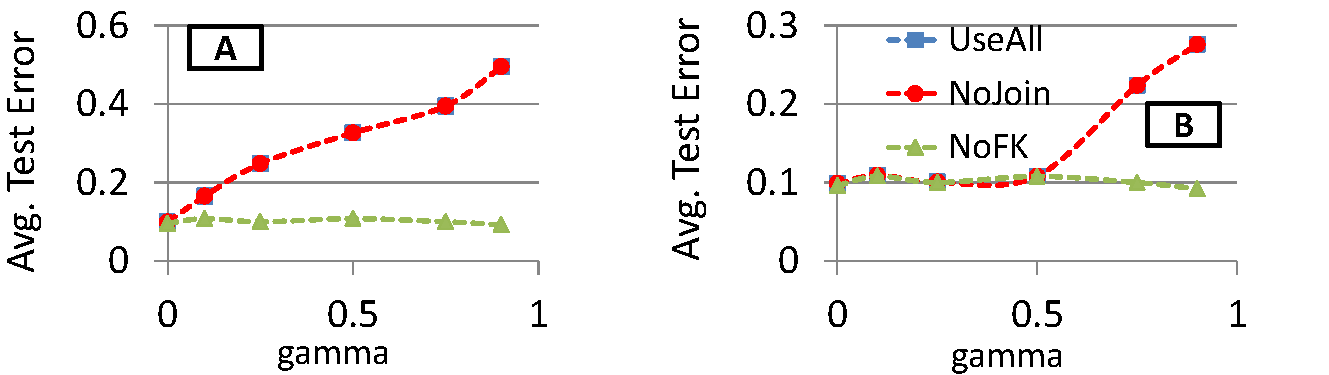
\includegraphics[width=0.99\linewidth]{smoothing.pdf}
\caption{Smoothing. (A) Random hashing. (B) $\textbf{X}_R$-based.}
\label{Figure:smoothing}
\end{figure}

The intuition for $\textbf{X}_R$-based smoothing is that if $\textbf{X}_R$ is part of the ``true'' distribution, it may yield higher accuracy 
than random reassignment. But if $\textbf{X}_R$ is just noise, this becomes essentially random reassignment.
To validate our claim, we use the OneXr simulation scenario. Recall that a feature $X_r \in \textbf{X}_R$
determines the target (with some Bayes noise as before). We introduce a parameter $\gamma$ that is the ratio of the number of $FK$ values not seen 
during training to $|\mathcal{D}_{FK}|$. If $\gamma = 0$, no smoothing is needed; as $\gamma$ increases, more smoothing is needed.
Figure~\ref{Figure:smoothing} presents the results. 

The plots confirm our intuition: the $\textbf{X}_R$-based smoothing yields much lower test errors for both \textit{NoJoin} and \textit{JoinAll} -- in 
fact, errors comparable to \textit{NoFK} and the Bayes error -- for lower values of $\gamma$ ($<0.5$). But as $\gamma$ gets closer to $1$, the 
errors of $\textbf{X}_R$-based smoothing also increase but not as much as random hashing. Overall, these results suggest that even if foreign features 
are available, rather for using them directly for learning the model, we could use them as side information for smoothing $FK$ features. In conclusion,
this approach suggests that it is possible to get ``the best of both worlds'': the runtime and usability gains of \textit{NoJoin} (as against \textit{JoinAll}, 
which unnecessarily also learns over the foreign features) along with exploiting the extra information provided by foreign features (if they are available)
for smoothing foreign key features. Of course, there are still many open questions on how best to exploit KFKDs and dimension tables, both methodological
and theoretical, and we have outlined some in this paper. We hope our analyses and results help spur more research in this direction.


\section{Related Work}

% We discuss the relationship of our work to key prior work from both the database, data mining, and ML literatures.

\paragraph*{Database Dependencies and ML}
The scenario of learning over joins of multiple tables without materializing the output of the join was studied in~\cite{orion,olteanuf,rendle,santoku},
but their goal was primarily to reduce runtimes of some ML techniques without affecting accuracy.
In contrast, our work focuses on the more fundamental question of whether foreign features are even needed for accuracy in the first place for complex ML models
such as decision trees and RBF-SVMs.
We first demonstrated the feasibility of discarding foreign features for linear VC dimension models such as logistic regression and Naive Bayes in~\cite{hamlet}.
In this work, we revisit that idea by demonstrating that popular infinite VC dimension models are counter-intuitively \textit{more} robust than linear models to avoiding 
foreign features, not \textit{less} as our VC dimension-based analysis in~\cite{hamlet} suggested. Further, we also evaluate mechanisms to make foreign key features more practical.
Embedded multi-valued dependencies (EMVDs) are database dependencies that are more general than functional dependencies~\cite{dbtheorybook}. 
The implication of EMVDs for probabilistic conditional independence in Bayesian networks was originally described by~\cite{pearl} and further explored by~\cite{wong}.
However, their use of EMVDs still requires computations over all features in the data instance. In contrast, our work demonstrates the dramatic effects of KFKDs and FDs 
in enabling us to avoid entire sets of features for complex ML models \textit{without performing any computations} on the foreign features.
There is a large body of work on statistical relational learning (SRL) to handle joins that cause duplicates in the fact table~\cite{srlbook}. But as mentioned before, 
our work focuses on the regular IID setting for which SRL might be an overkill.

\paragraph*{Feature Selection}
The data mining and ML communities have long studied the problem of feature selection to improve ML accuracy~\cite{guyonbook,hastie}.
In contrast, our goal is \textit{not} to design new feature selection methods. Rather, we want to demonstrate that foreign features quite often do not help improve 
accuracy when learning some popular complex ML classifiers. This can be viewed as a way of ``short-circuiting'' the feature selection process using database schema 
information, with the aim of obviating large amounts of computations over foreign features.
The trade-off between feature redundancy and relevancy is well-studied~\cite{guyonbook,leiyu,daphnekoller}. The conventional wisdom is that even a feature that is 
redundant might be highly relevant and hence, unavoidable in the mix~\cite{guyonbook}. Our work establishes, perhaps surprisingly, that this is \textit{not} the case 
for foreign features; even if a foreign feature is highly relevant, it can be safely discarded in most practical cases for decision trees and RBF-SVMs.
There is prior work on exploiting FDs in feature selection.
\cite{approxfds} infers approximate FDs using the dataset instance and exploits them during feature selection.
FOCUS~\cite{focus} is an approach to bias the input and reduce the number of features by performing some computations over those features.
Our work is orthogonal to all of these approaches that require computations over all features because we show that FDs caused by KFK joins imply that foreign features 
can often be discarded when learning complex ML models \textit{without even looking at the features} and obviously, without performing any computations on them!
To the best of our knowledge, no feature selection method exhibits such a dramatic capability that our work opens up.
Scores such as Gini and information gain are known to be biased towards large-domain features in decision tree learning~\cite{dtreebias1} and different approaches 
have explored alternatives to solve that issue~\cite{dtreebias2}. Our problem is orthogonal because we focus on how FDs enable us to ignore foreign features a priori 
without affecting accuracy significantly. Furthermore, even with the gain ratio score that mitigates the bias towards large-domain features, our main findings stand.
Unsupervised dimensionality reduction methods such as random hashing or PCA are also popular~\cite{hastie,mitchellbook}. Our lossy compression techniques to 
reduce the domains of foreign key features for decision trees are inspired by such methods.

TODO: More citations, discussions

\paragraph*{ML and Analytics Benchmarks}

TODO: More citations, discussions


\section{Conclusion and Future Work}


\pagebreak

\bibliographystyle{abbrv}
\bibliography{HamletVLDB}

\end{document}